\documentclass[acmlarge]{acmart}

\usepackage{booktabs} % For formal tables
\usepackage{comment}
\usepackage{color}
\usepackage{soul}
\usepackage{hyperref}
\usepackage{url}
\usepackage{multirow}
\usepackage{subfigure}

\usepackage{amsmath}
%\usepackage{algorithm}
%\usepackage[noend]{algpseudocode}
\usepackage[lined,linesnumbered,ruled]{algorithm2e}
\usepackage[flushleft]{threeparttable}

\def\sectionautorefname{Section}
\def\figureautorefname{Figure}
\def\subfigureautorefname{Figure}
\def\tableautorefname{Table}
\def\algorithmautorefname{Algorithm}
\def\equationautorefname{Eqn.}

\newtheorem{Def}{Definition}[section]
%\def\definitionautorefname{Definition}
\newcommand{\Defautorefname}{Definition}

\def\on{{on}}
\def\off{{o\!f\!f}}
\def\dist{\mathrm{dist}}
\DeclareMathOperator{\tr}{tr}
\DeclareMathOperator{\proj}{proj}

\newcommand{\ie}{i.e., }
\newcommand{\eg}{e.g., }
\newcommand{\note}[1]{\textbf{\color{red}[***** #1 *****]}}
%\renewcommand{\note}[1]{}

\newtheorem{case}{Use Case}
%\newtheorem{example}{Example}

%\usepackage[ruled]{algorithm2e} % For algorithms
\renewcommand{\algorithmcfname}{ALGORITHM}
\SetAlFnt{\small}
\SetAlCapFnt{\small}
\SetAlCapNameFnt{\small}
\SetAlCapHSkip{0pt}
\IncMargin{-\parindent}

% Metadata Information
%\acmJournal{JOCCH}
%\acmVolume{9}
%\acmNumber{4}
%\acmArticle{39}
%\acmYear{2010}
%\acmMonth{3}
%\acmArticleSeq{11}

%\acmBadgeR[http://ctuning.org/ae/ppopp2016.html]{ae-logo}
%\acmBadgeL[http://ctuning.org/ae/ppopp2016.html]{ae-logo}


% Copyright
%\setcopyright{acmcopyright}
%\setcopyright{acmlicensed}
%\setcopyright{rightsretained}
%\setcopyright{usgov}
\setcopyright{usgovmixed}
%\setcopyright{cagov}
%\setcopyright{cagovmixed}

% DOI
%\acmDOI{0000001.0000001}

% Paper history
%\received{February 2007}
%\received{March 2009}
%\received[accepted]{June 2009}


% Document starts
\begin{document}
% Title portion
\title{Inferring Correlation between User Mobility and App Usage in Massive Coarse-grained Data Traces}

\author{Zheng Lu}
\affiliation{%
  \institution{University of Tennessee}
  \department{Electrical Engineering and Computer Science}
}
\email{zlu12@vols.utk.edu}
\author{Yunhe Feng}
\affiliation{%
  \institution{University of Tennessee}
  \department{Electrical Engineering and Computer Science}
	%\email{yfeng14@vols.utk.edu}
}
\author{Wenjun Zhou}
\affiliation{%
	\institution{University of Tennessee}
  \department{Business Analytics \& Statistics}
	%\email{wzhou4@utk.edu}
}
\author{Xiaolin Li}
\affiliation{%
  \institution{Nanjing University}
  \department{School of Management}
	%\email{lixl@nju.edu.cn}
}
\author{Qing Cao}
\affiliation{%
  \institution{University of Tennessee}
  \department{Electrical Engineering and Computer Science}
	%\email{cao@utk.edu}
}


\begin{abstract}
With the rapid growth in smartphone usage, it has been more and more important to understand the patterns of mobile data consumption by users.
In this paper, we present an empirical study 
of the correlation between user mobility and app usage patterns.
In particular, we focus on users' moving speed as the key mobility metric,
and try to answer the following question:
are there any notable relations between moving speed and the app usage patterns?
Our study is based on a real-world, large-scale dataset of 2G phone network data request records.
A critical challenge was that the raw data records are rather coarse-grained.
More specifically, unlike GPS traces, the exact locations of users were not readily available.
We inferred users' approximate locations according to their interactions with nearby cell towers, whose locations were known.
We %address the challenge of user speed estimation by 
proposed a novel method to filter out noises and perform reliable speed estimation.
We verify our methodology with out of sample data and show its improvement in speed estimation accuracy.
We then examined several aspects of mobile data usage patterns,
including the data volume, the access frequency, and the app categories,
to reveal the correlation between these patterns and users' moving speed.
Experimental results based on our large-scale real-world datasets revealed that users under different mobility category not only have different smartphone usage motivations but also have different ways of using their smartphones.
\end{abstract}


%
% The code below should be generated by the tool at
% http://dl.acm.org/ccs.cfm
% Please copy and paste the code instead of the example below. 
%
%\begin{CCSXML}
%<ccs2012>
 %<concept>
  %<concept_id>10010520.10010553.10010562</concept_id>
  %<concept_desc>Computer systems organization~Embedded systems</concept_desc>
  %<concept_significance>500</concept_significance>
 %</concept>
 %<concept>
  %<concept_id>10010520.10010575.10010755</concept_id>
  %<concept_desc>Computer systems organization~Redundancy</concept_desc>
  %<concept_significance>300</concept_significance>
 %</concept>
 %<concept>
  %<concept_id>10010520.10010553.10010554</concept_id>
  %<concept_desc>Computer systems organization~Robotics</concept_desc>
  %<concept_significance>100</concept_significance>
 %</concept>
 %<concept>
  %<concept_id>10003033.10003083.10003095</concept_id>
  %<concept_desc>Networks~Network reliability</concept_desc>
  %<concept_significance>100</concept_significance>
 %</concept>
%</ccs2012>  
%\end{CCSXML}
%
%\ccsdesc[500]{Computer systems organization~Embedded systems}
%\ccsdesc[300]{Computer systems organization~Redundancy}
%\ccsdesc{Computer systems organization~Robotics}
%\ccsdesc[100]{Networks~Network reliability}

%
% End generated code
%

%% We no longer use \terms command
%\terms{Design, Algorithms, Performance}
%
%\keywords{Wireless sensor networks, media access control,
%multi-channel, radio interference, time synchronization}
%
%
%\thanks{This work is supported by the National Science Foundation,
  %under grant CNS-0435060, grant CCR-0325197 and grant EN-CS-0329609.
%
  %Author's addresses: G. Zhou, Computer Science Department, College of
  %William and Mary; Y. Wu {and} J. A. Stankovic, Computer Science
  %Department, University of Virginia; T. Yan, Eaton Innovation Center;
  %T. He, Computer Science Department, University of Minnesota; C.
  %Huang, Google; T. F. Abdelzaher, (Current address) NASA Ames
  %Research Center, Moffett Field, California 94035.}


\maketitle

% The default list of authors is too long for headers}
\renewcommand{\shortauthors}{Z. Lu et al.}

\section{Introduction}\label{intro}

In the past decade, the use of smartphones has grown significantly among consumers.
According to a recent report~\cite{Ericsson}, there are 3.4 billion smartphone users worldwide,
and the accumulated mobile data traffic has reached 120 exabytes in 2015.
One critical reason for this explosive growth is the popularity of smartphone apps,
such as those served by Google Play and Apple Store,
whose number has exceeded 1.5 million by July 2015~\cite{Statista}.
It is estimated that people spend as much as 30 hours monthly on these apps on average,
a growth of over 65 percent compared to 2013~\cite{Nielsen}.

Consequently, recent research has invested considerable effort to understand smartphone app usage behavior,
as such understandings can help app developers and mobile advertisers tremendously~\cite{xu2011identifying,yang2015characterizing}.
In the previous work, both temporal patterns (\eg individual app usage histories) and
spatial patterns (\eg location contexts) have been extensively studied~\cite{meng2014analyzing}.
Their results have enabled novel applications,
such as smartphone app launching prediction services~\cite{yan2012fast}
and location-aware event recommendations.

In this paper, we focus on one less investigated feature, user mobility,
and investigate how this feature correlates with the usage patterns of smartphone app users.
Understanding such correlations, if any, could provide useful contextual information
for relevant and accurate app recommendation and ad delivery.
For example, if we find out hiking hobbyists use certain apps considerably more often,
then such apps may be more useful venues for ad delivery for equipment makers for hiking activities.

Unfortunately, previous work on this topic has only investigated this problem in highly limited and controlled contexts,
and by taking account into the usage history of a small set of users.
For example, a few works have addressed the problem of transportation mode inference,
where the goal is to find out whether a user is riding a bus or taking a taxi, among other possibilities.
Such work usually assumes that additional hardware (\eg GPS, sensors) is available,
and is carried out for a small group of users in controlled experiments~\cite{6958169, 6450942, zheng2010understanding, biljecki2013transportation, stenneth2011transportation, 5283030, 6460199, Reddy:2010:UMP:1689239.1689243}.
Later work suggested that it may be possible to use cell tower communications to monitor users' mobility indirectly~\cite{rose2006mobile},
where efforts have been focusing on inferring users' trajectories~\cite{Alsolami2012Auth,jiang2013review}
or transportation mode~\cite{wang2010transportation,bekhor2015investigation} only using cell-phone traces
(\eg Call Detail Records, handover data) that do not directly contain location information.
Such approaches are more scalable, as they do not require additional hardware resources and better respect users' privacy.
The limitations of these approaches, however, are that they are usually small-scale by nature, and
usually has ground-truth data collected for a user as validation methods for their approaches.

Our work is following this latter line of research of using large-scale cell-phone tower traces.
However, our dataset and the corresponding methodology are significantly different.
First, our dataset consists of a truly large population,
where we have access to mobile data access histories of millions of users in three cities that cover thousands of square miles.
The number of users is perhaps more than the population of certain countries in the world.
Second, due to privacy concerns, the dataset is fundamentally coarse-grained,
meaning that we do not, and can not, collect the ground truth information for these millions of users.
Therefore, novel data processing methods are urgently needed.
Finally, our research goals are to reveal large-scale, population-level correlations,
if any, between user mobility and app usage patterns,
a goal that has not been addressed in any of previous research work.
We emphasize, however, due to the second limitation on the absence of ground truth,
all our conclusions are, at best, educated guesses that are based on real-world data.
We believe such results are meaningful and insightful for a wide range of target people:
app developers, ad distributors, network operators, and end users.

We address the following two challenges in our work.
First, to infer user mobility with cell-phone traces,
we need to filter the location history to obtain accurate estimates. In our dataset, the only location information available is the communication history between a customer and a cell tower. Fortunately, we have the precise locations of each cell towers, and by communication principles, we know that a user's phone typically contacts the tower with the best signal reception (usually the nearest one). We have surveyed the previous work on estimating trajectories based on similar datasets~\cite{smoreda2013spatiotemporal, hoteit2014estimating, widhalm2015discovering, Alsolami2012Auth, jiang2013review} or finding mobility motifs~\cite{wang2014mobile, gambs2012next}, but we could not find one that suits our needs as we find their results are clearly still too coarse-grained. One reason is the dataset difference: their data mostly are sparse compared to ours. For example, one dataset contains users who perform daily commute or city to city long distance trips. In contrast, our data are in dense urban areas where users employ a mixture of transportation modes ranging from walking, bicycles, to buses and cars. Railway transportation is not present in our dataset. Therefore, based on these concerns, we need to develop a novel methodology to estimate more complicated and fine-grained user mobility trajectories for our target dataset.

Second, to correlate the usage history of apps with mobility patterns successfully, we need to develop a tradeoff between the most popular apps and sparsely distributed ones. More precisely, we find that a majority of users will use those ``heavy-hitter'' apps no matter what their mobility patterns are. Therefore, inferring such correlations are less meaningful. Instead, we should focus on those app groups where data exhibit differentiated popularity for various groups of users with different moving speeds, a task that is considerably more challenging than simply performing correlation analysis between all apps and users without differentiation. Therefore, our methods need to be customized for the needs of this application analysis task.

The main contributions of this paper can be summarized as follows.
%\begin{itemize}
%	\item 
We design and evaluate a novel methodology to infer user speeds with cell-phone traces with low location accuracies. Compared to existing approaches, this methodology achieves far better and fine-grained estimation with adjustable confidence levels. Specifically, to overcome the problem of location accuracy, our methodology involves steps to segment traces by pass-boundary events, i.e., when a user establishes a new connection with a different tower, and performs intra-cell level zooming and analysis to calculate distance estimates. This method is also robust against issues caused by the uncertain nature of wireless communications, \eg a user located in the overlapped communication coverage area of multiple towers may randomly communicate with each tower, causing cell oscillations that other simple methods cannot easily address.
%	\item 
With the more accurate speed estimates, we are able to study the correlation of user mobility with app usage patterns in a population in an uncontrolled, real-world environment. The results are novel in that no previous work, to the best of our knowledge, has gained similar insights or reported findings in this aspect. Our revealed correlations of user speed and mobile data access patterns include the data volume, the access frequency, the share of each smartphone app category in the total mobile data traffic, and user preferences of apps under different transportation modes.
%\end{itemize}

The rest of this paper is organized as follows.
In Section~\ref{relate}, we describe previous works on user mobility inference and geospatial app usage patterns.
Section~\ref{data} defines our problem and provides details on the mobile data access trace we use in this paper.
We describe our speed estimation methodology and design in Section~\ref{approach}.
Section~\ref{experiments} explains our findings on the correlation of user speeds and mobile data access patterns.
Finally, we conclude our work in Section~\ref{conclusion}.


\begin{figure*}
  \centering
  \subfigure[Number of Records       \label{fig:data_stat1}]{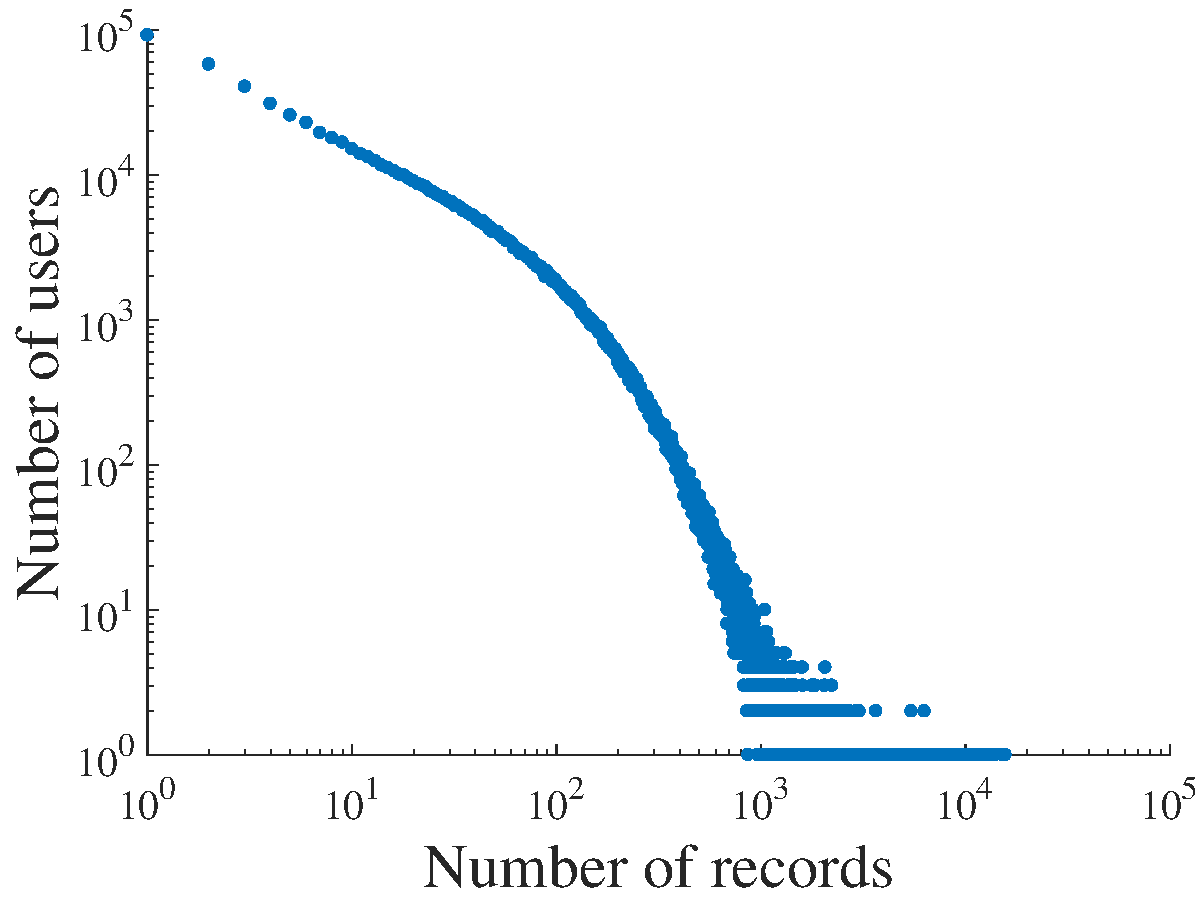
\includegraphics[width=0.32\textwidth]{figures/record_count_hist.pdf}}
  \subfigure[Avg. Time Interval      \label{fig:data_stat2}]{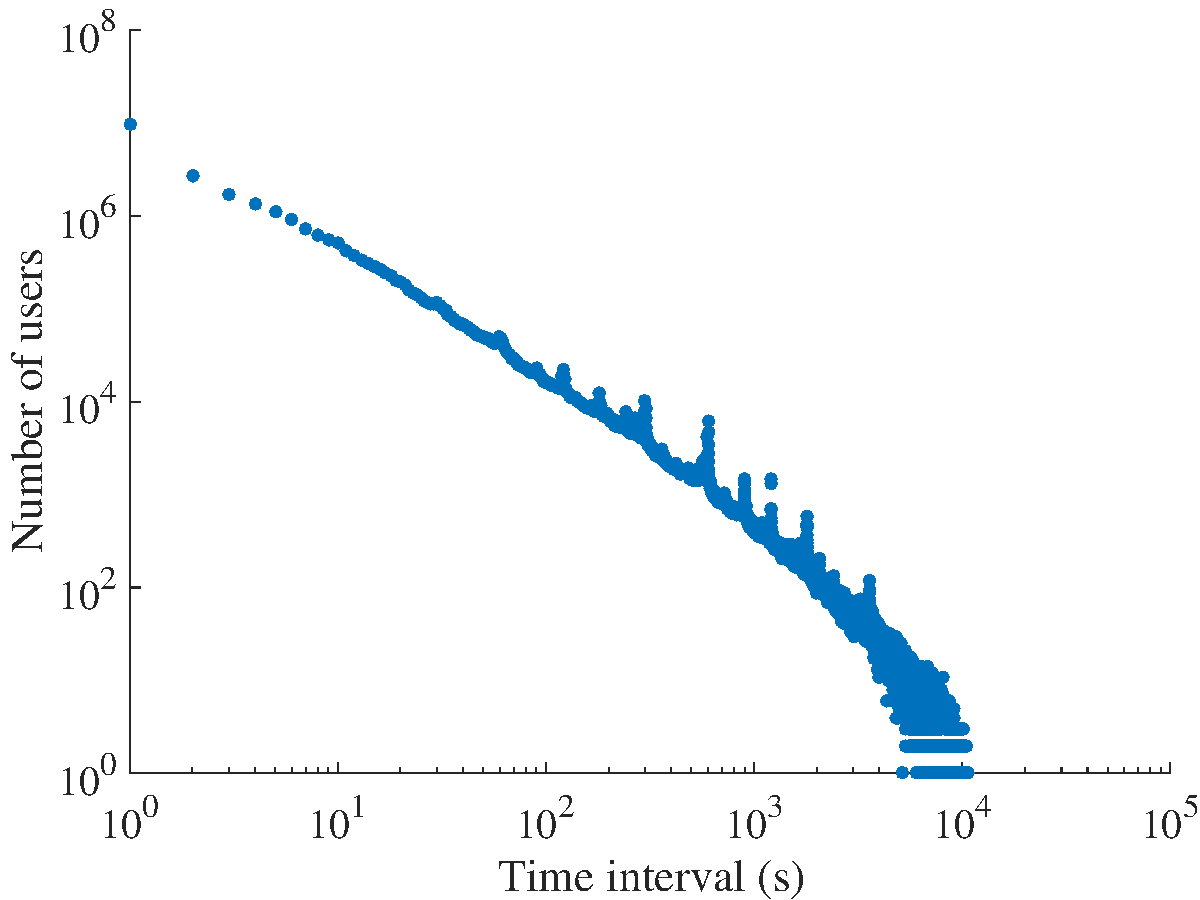
\includegraphics[width=0.32\textwidth]{figures/time_interval_hist.pdf}}
  \subfigure[Number of Towers Visited\label{fig:data_stat3}]{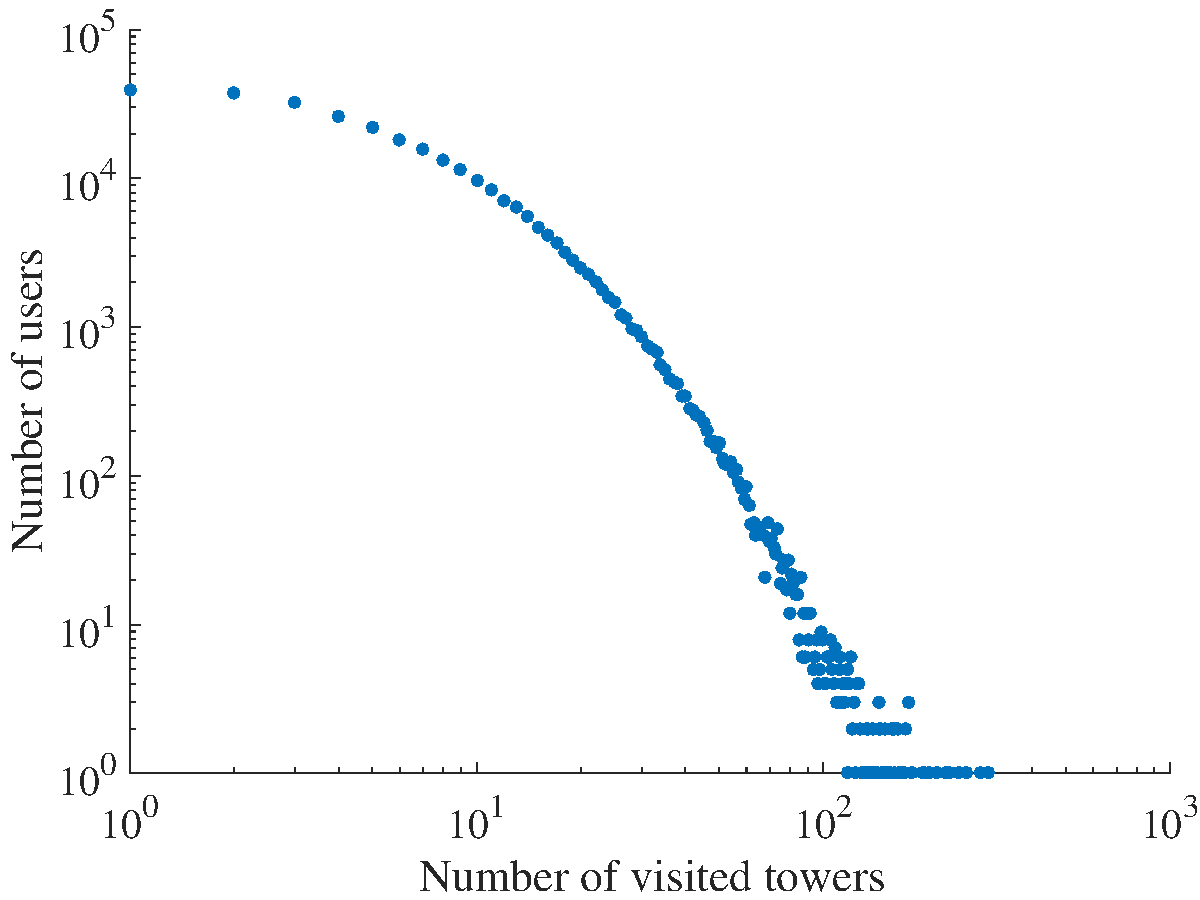
\includegraphics[width=0.32\textwidth]{figures/visited_tower_hist.pdf}}
  \vspace{-0.1in}
  \caption{Dataset characteristics.}\label{fig:data_stat}
  \vspace{-0.1in}
\end{figure*}


\section{Related Work}\label{relate}


In this section, we summarize recent literature on smartphone apps, user mobility, and geospatial analysis of mobile phone apps data.


%\subsection{Smartphone Apps}

To study the smartphone app usage behavior of a large group of users, previous work has analyzed mobile data traces generated by smartphone apps in studies of various scales. \cite{yang2015characterizing} studied the mobile user behavior by focusing on data usage, mobility pattern and application usage. In \cite{xu2011identifying}, the aggregated spatial and temporal prevalence, locality and correlation of smartphone apps at a national scale is investigated, by analyzing the mobile data generated by smartphone apps. \cite{bohmer2011falling} performed a deployment-based study over 4,100 users of Android mobile devices and showed both basic app usage patterns and contextual app usage patterns. Unlike our work, these previous work have not studied the relation of mobile user behavior with more complex user mobility, \ie user speed.

%\subsection{User Mobility}

Using GPS~\cite{ohashi2014automatic, ryder2009ambulation, zheng2010understanding, biljecki2013transportation, stenneth2011transportation, waga2012detecting, widhalm2012transport, Reddy:2010:UMP:1689239.1689243}
and embedded sensors~\cite{Hemminki:2013:ATM:2517351.2517367, wang2010accelerometer, shin2015urban, manzoni2010transportation, tacconi2011smartphone, Reddy:2010:UMP:1689239.1689243, ohashi2014automatic}, a separate body of research is able to use smartphones to infer user mobility patterns accurately in small-scale, controlled experiments, such as inferring transportation modes. Most of these works formulate the problem as a classification problem, where common challenges involve data segmentation ~\cite{ohashi2014automatic,waga2012detecting, zheng2010understanding, biljecki2013transportation}, feature selection~\cite{zheng2010understanding, biljecki2013transportation, wang2010accelerometer, stenneth2011transportation}. Multiple methods, such as SVM or linear regressions, are developed to achieve the best accuracy. 

Although GPS and sensors are well suited for small-scale experiments, they are not scalable as users typically do not want their GPS traces to be shared with others. In recent work~\cite{rose2006mobile},  it is revealed that there is a great potential for using cell-phone data traces such as Call Detail Records (CDRs) for user mobility inference. A large body of research literature exists applying this method for inferring user's trajectories ~\cite{smoreda2013spatiotemporal, hoteit2014estimating, widhalm2015discovering, Alsolami2012Auth, jiang2013review, bekhor2015investigation, leontiadis2014cells} or mobility motifs~\cite{wang2014mobile, gambs2012next}. For example, \cite{Alsolami2012Auth, jiang2013review} inferred user trajectories from cell-phone traces based on how likely a specific route can lead to similar tower access sequences stored in the data traces. In another work~\cite{wang2010transportation}, it aims to classify a user's transportation mode by clustering travel time distribution. Finally, researchers~\cite{bekhor2015investigation} also proposed approaches that can deal with common zig-zag problems in inferring user mobility from smartphone traces.
Different from these existing methods, however, our approach takes advantage of the scalability of cell-phone data traces and achieves fine-grained user mobility inference on top of it.

%\subsection{Geospatial App Usage}

Studying correlations between app usage and features extracted from phone traces is not new in the literature. Previous work has studied relations of human mobility and social networks using geospatial features. For example, a work \cite{cho2011friendship} found that the short-ranged travels are periodic and not likely to be related to the social network structures, while long-distance travels are heavily related to the social network status of a user. Based on these findings, a model was proposed to predict dynamics of future human movement with a high accuracy. Follow-up works such as~\cite{Noulas11} studied a similar problem with a different dataset. ~\cite{shafiq2012characterizing,yang2015characterizing} studied the geospatial relation of the app usage volume. Their works mostly studied the spatial correlation of the smartphone usage, while the user mobility's impact on app usage is still a missing piece of these works. ~\cite{meng2014analyzing} studied how the proximity, the location and individual differences (e.g., personality) can affect the user's mobile data usage. Finally, ~\cite{yang2016apps} showed the apps access pattern under various user mobility properties such as the number of visited cell phone towers and the radius of gyration. However, analysis of much complex user mobility such as user speed is still a missing piece in these works. 

Another aspect addressed in the literature is related to the tradeoffs adopting either cellular network data or WiFi data. Although recent studies ~\cite{lee2010mobile,baumann2014availability} have shown that WiFi handles half of the mobile data traffic, it has been observed that cell phone networks typically have much better coverage and user mobility diversity~\cite{wagner2014device, yadav2014characterizing}. Furthermore, it is practically impossible to collect city-level WiFi data due to the heterogeneous nature of access points and privacy concerns. Therefore, it is more meaningful to study large-scale user mobility under cellular traffic, as is the methodology followed by this paper.

\section{Problem Setting}\label{data}

In this section, we provide a description of the dataset,
followed by an example of a user's data.

\subsection{Dataset Description}

Our dataset contains mobile data access history of all active users (during a three-hour period)
of a major mobile carrier in three cities of China.
For each user, all data request records during the study period are available,
where each record consists of the user ID (a hashed value for anonymity), 
the tower ID (from which we were able to look up its geo-coordinates), 
the timestamp, 
the app identifier, 
and other data access features such as data volumes.

%the following information:
%\begin{description}
%  \item[User ID]: the identifier of a user, a hashed value for anonymity;
%  \item[Tower Location]: the geo-coordinates of a cell phone tower with which a user has established handshake and communicated; %, denoted by $l$.
%  \item[Timestamp]: the Timestamp consists of the date and time of a mobile data access record; %, denoted by $t$.
%  \item[Data Access Features]: contain the app identifier that initiates the data communication, and data volumes.
%  %\item ... represents many other attributes not of focus here.
%\end{description}
%%Note that one app may initiate multiple data transaction records to complete one data transfer in practice, depending on the signal strength and packet deliveries success ratios.

\begin{figure}[h]
    \centering
    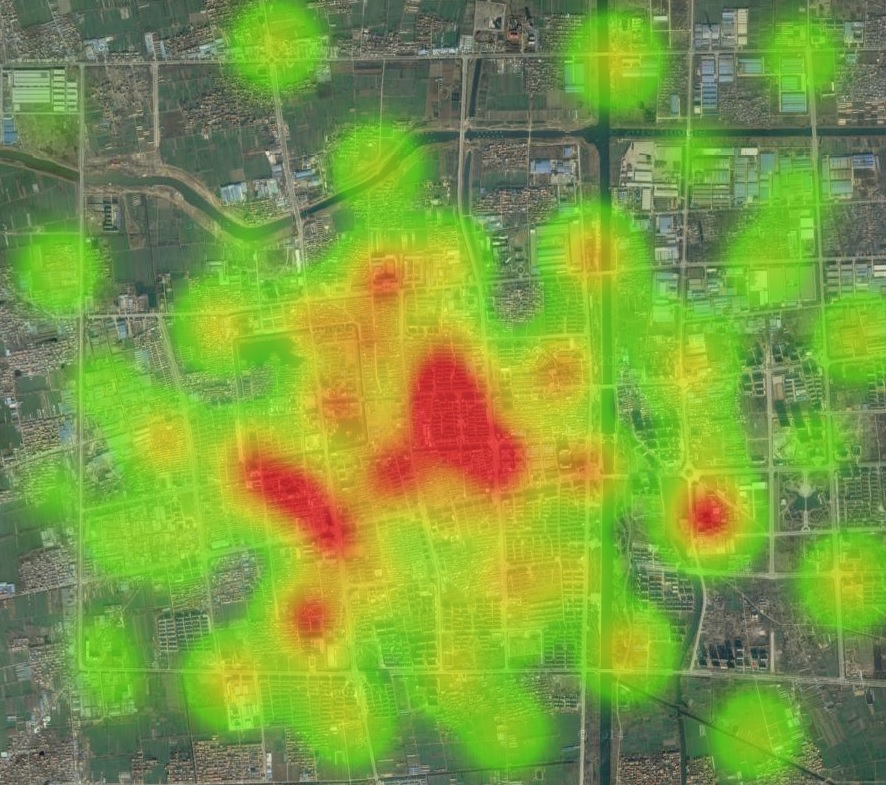
\includegraphics[width=0.8\linewidth]{./figures/hotmap.jpg}
    %\vspace{-0.1in}
    \caption{Communication density in a city area.}
    \label{fig:city_sample} 
    \vspace{-0.1in}
\end{figure}

%%Before proceeding to the details of our approaches, we briefly introduce our dataset in this section.
%The dataset is a collection of the aforementioned mobile data access records provided by a cellular network operator in China, collected from  three mid-size cities, including both urban and suburban areas, during a three-hour period in the early evening (6pm - 9pm) in 2014. The cities are anonymous in this paper. 
The dataset includes more than 58 million mobile data access records with a total volume of more than 720 gigabytes, which covers all cell phones that were actively exchanging data with a total of 5199 cell towers in the area during the observation period. 
The number of unique users included in this dataset is identified as around 900 thousand. % removing duplicates. 
The total active time of all users accumulates to more than 1 million hours. 
\autoref{fig:city_sample} shows a heatmap of the mobile data access in a city area of our dataset.

\subsection{Data Preprocessing Findings}

%We first preprocess the dataset and we have the following preliminary findings.
We first preprocess the data and analyze the characteristics of mobile data access patterns.  % of each individual in our study,
Distributional characteristics are visualized in \autoref{fig:data_stat}.
In particular,
the number of records per user,
the average time intervals between consecutive records, and
the number of towers visited.
%the contribution of each category of apps on total mobile data traffic.
We found that our dataset has a highly skewed distribution of
the number of records per user, as shown in \autoref{fig:data_stat1}, and
the time intervals between consecutive records, as shown in \autoref{fig:data_stat2}.
Here, a higher record density, \ie more records for a user in a time unit, indicates a better performance to infer user mobility even when the trip length is very short,
as we can obtain a better granularity by analyzing these records.
Actually, it is the case that most user only traveled a very short trip in terms of the number of visited towers according to \autoref{fig:data_stat3}.

\begin{figure*}
    \centering
    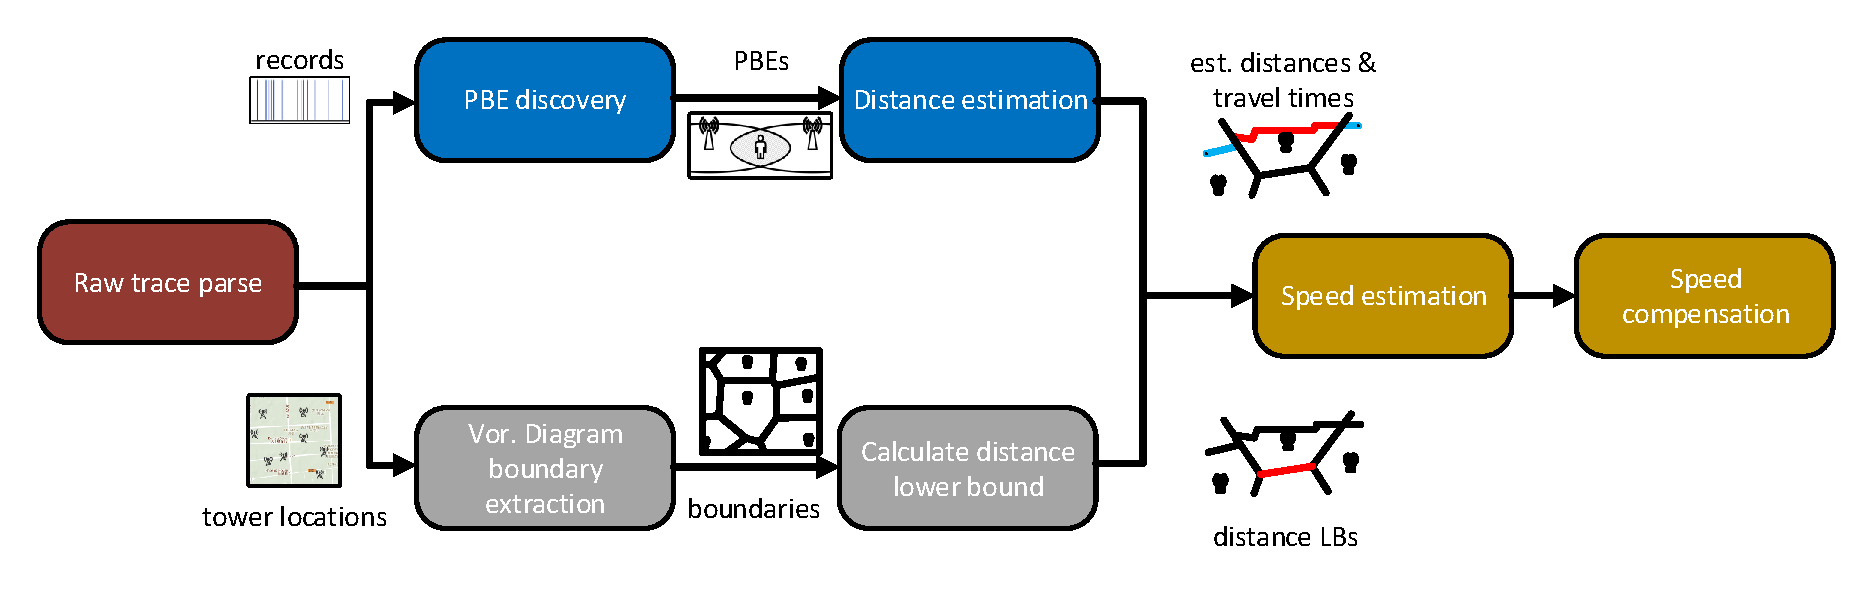
\includegraphics[width=\linewidth]{./figures/system_overview.pdf}
    \vspace{-0.4in}
    \caption{Speed estimation system overview.}
    \label{fig:system_overview}
    \vspace{-0.1in}
\end{figure*}

Note that our dataset differs from commonly used mobility datasets used in existing work.
Compared to moving trajectories like those captured by GPS,
we do not know the exact locations of the users, and we only know a user is located nearby a tower to communicate with it.
Furthermore, compared to other datasets with call detail records (CDR),
our dataset is drawn from a region with more densely populated customers, where each may adopt different mobility methods such as walking, driving, or taking buses.
Such differences make it harder to accurately estimate user speed based on existing methods. %For example...


\subsection{An Example User's Traces}

To provide a clear view of our data, we visualize a user's records from our dataset in \autoref{fig:typical_user} as a running example.

\begin{figure}[h]
    \centering
    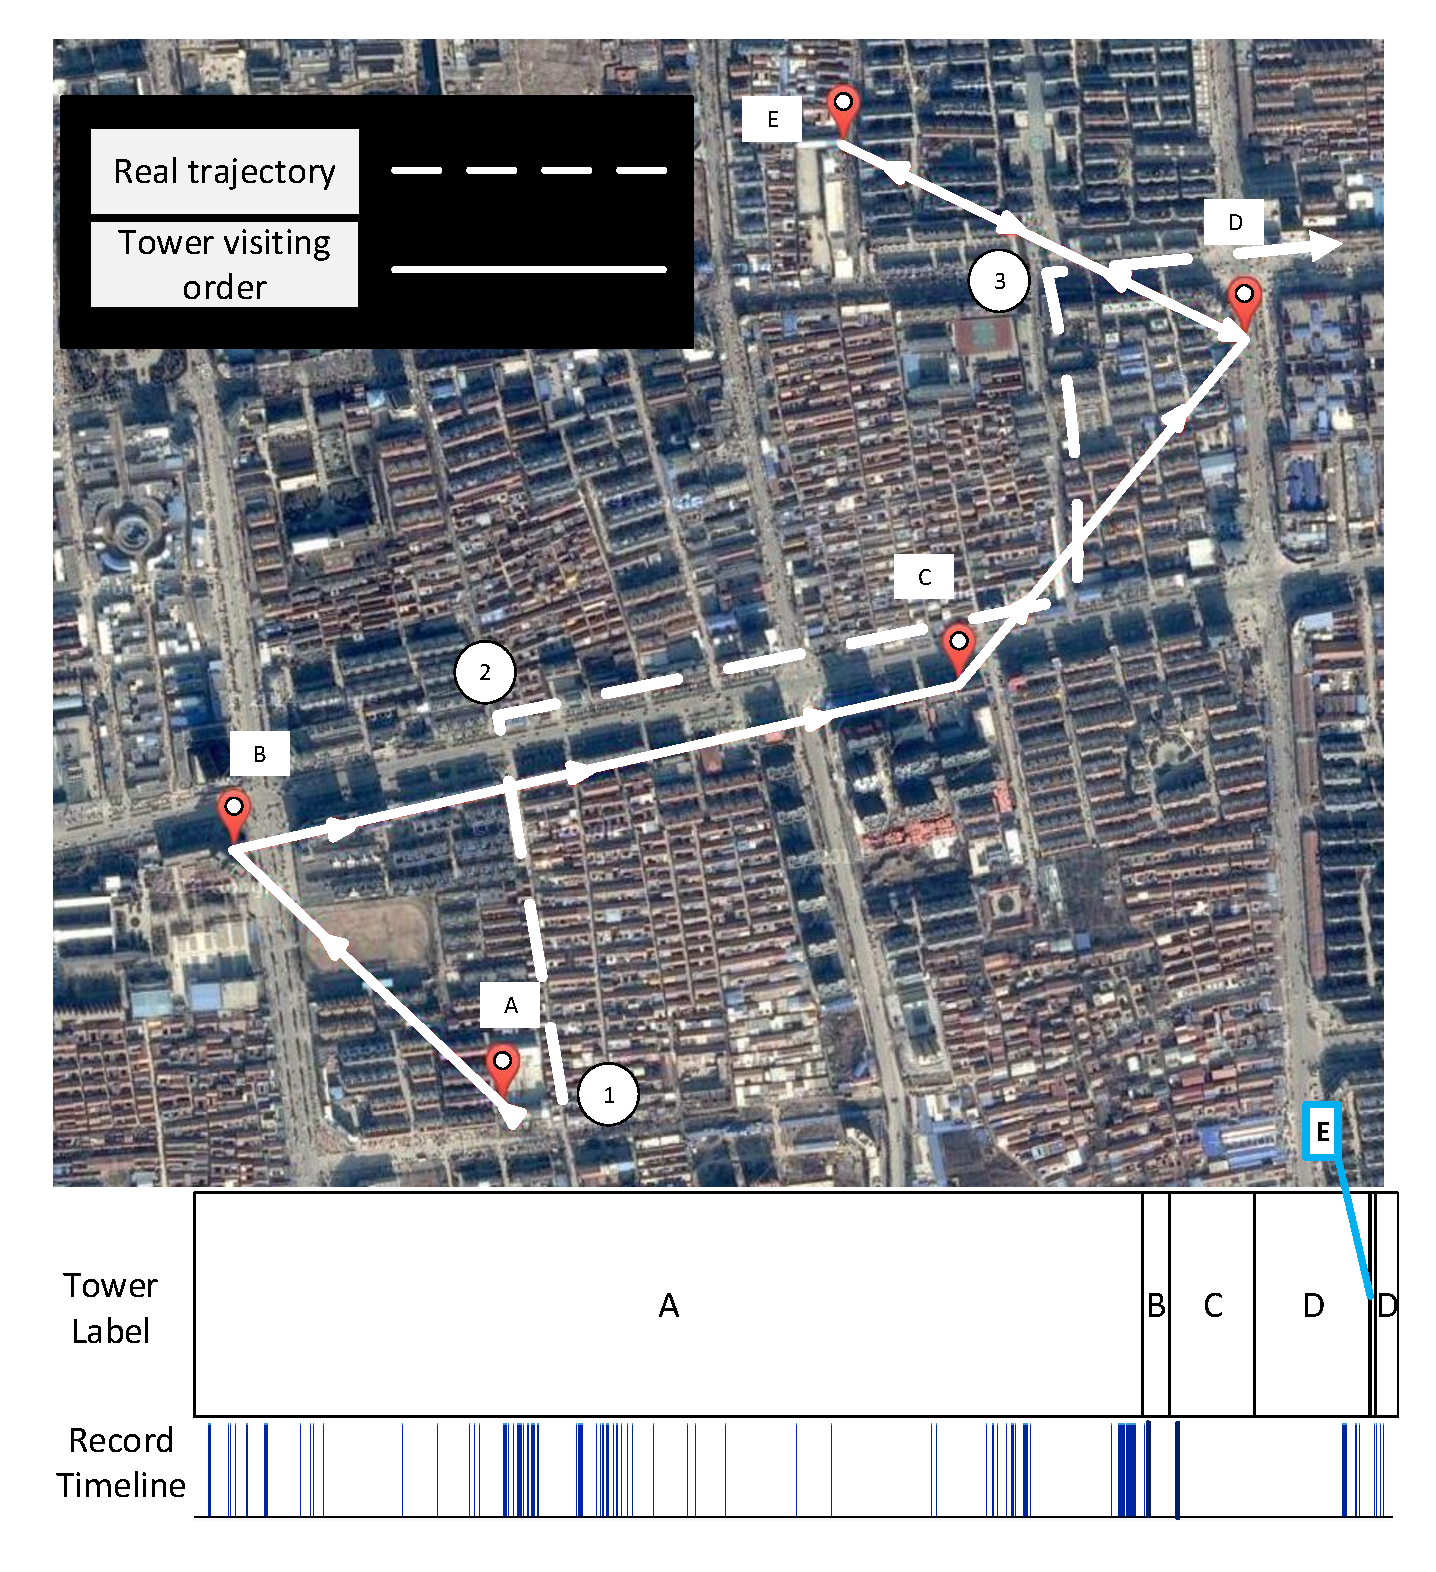
\includegraphics[width=\linewidth]{./figures/typical_user.pdf}
    \vspace{-0.3in}
    \caption{Example data access activities of a user.}
    \label{fig:typical_user}
    \vspace{-0.1in}
\end{figure}

Suppose that the user was taking the path (while using the cell phone) shown with the dashed line.
In particular, she started by walking from location 1, to location 2 where she waited for the bus.
After a few minutes, she got onto the bus, which took the path towards location 3.
Even though we did not know the actual path of the user,
her locations could be inferred by the nearby towers to which her communication data were sent to.


Since the cell tower locations are all known,
we can display the tower locations on a map that were visited by the user.
%Although we do not have the ground truth of user trajectory, for the sake of the example,
We use markers to show tower locations and arrowed lines to show the sequence of visiting.

The bottom part of \autoref{fig:typical_user} shows the timeline of the user's data access records with pulses.
We also show with which tower the user has communicated for each mobile data access record, by providing tower labels above the pulses.
Therefore, for this particular user, she communicated with tower A for a quite long time,
and shortly connected to tower B before switching to tower C.
After a while, the user was found in tower D's coverage area.
Then she connected to tower E for a very short time as location 3 is equally close to both tower C and tower D, \ie a possible cell oscillation, and in the end switched back to tower D.




\section{Speed Estimation}\label{approach}
%Estimating User Mobility Speeds with Coarse Data Records

In this section, we systematically describe our methodology for estimating user mobility speed using coarse-grained tower communication records and timestamps.

\subsection{Methodology Overview}

Our methods consist of multiple steps, where we first decompose traces of each user into segments to zoom into intra-cell speed estimation. Next, we estimate the distance and the travel time for each segment, where we employ a distance lower bound to filter out low-confidence estimates. In practice, such estimates are usually too noisy to be meaningful or reliable. Finally, we demonstrate how to compensate for speed estimation errors. \autoref{fig:system_overview} shows the structural overview of this methodology. The raw data parser on one end of this figure gathers data access records by users and sorts records of each user by time. On the other end, a list of tower locations from the mobile data access traces is extracted. Note that the system assigns a list for each city during processing steps.

After we have parsed raw traces, we next process them in different steps in parallel. In one of the next steps, we analyze traces of each user and generate pass-boundary events (PBEs) with the timestamp and location estimates of each record. Based on these events, we can estimate intra-cell travel distances and time accordingly.

In the second sequence of steps, we process the tower list for each city, by generating a Voronoi diagram based on tower coordinates. Here, Voronoi diagrams are used to simulate the tower coverage map, based on which we calculate all intra-cell boundary-to-boundary distance lower bounds. We keep such bounds in a separate list for lookup needs.

Finally, at the end of both processing sequences, we aggregate their results to estimate each user's speed distributions. We observe that for some segments, we do not have sufficient location information to accurately estimate a particular user's speed. Under such scenarios, we develop a compensation step where we try to infer the most likely speed based on speed distributions of this user in adjacent segments. The assumption is that one user will not change speed too much in short distances. We next discuss each component in more details in the following sections.

\subsection{Pass-Boundary Events}

%As our dataset is coarse-grained, we only have location information of the towers with which a user communicates. 
As a user could be anywhere inside the tower's coverage area, we need to infer their speeds by exploiting multiple coverage areas. To this end, we first decompose the trace into segments, which we call ``pass-boundary events'' (PBE).

\begin{figure}[h]
    \centering
    %\vspace{-0.1in}
    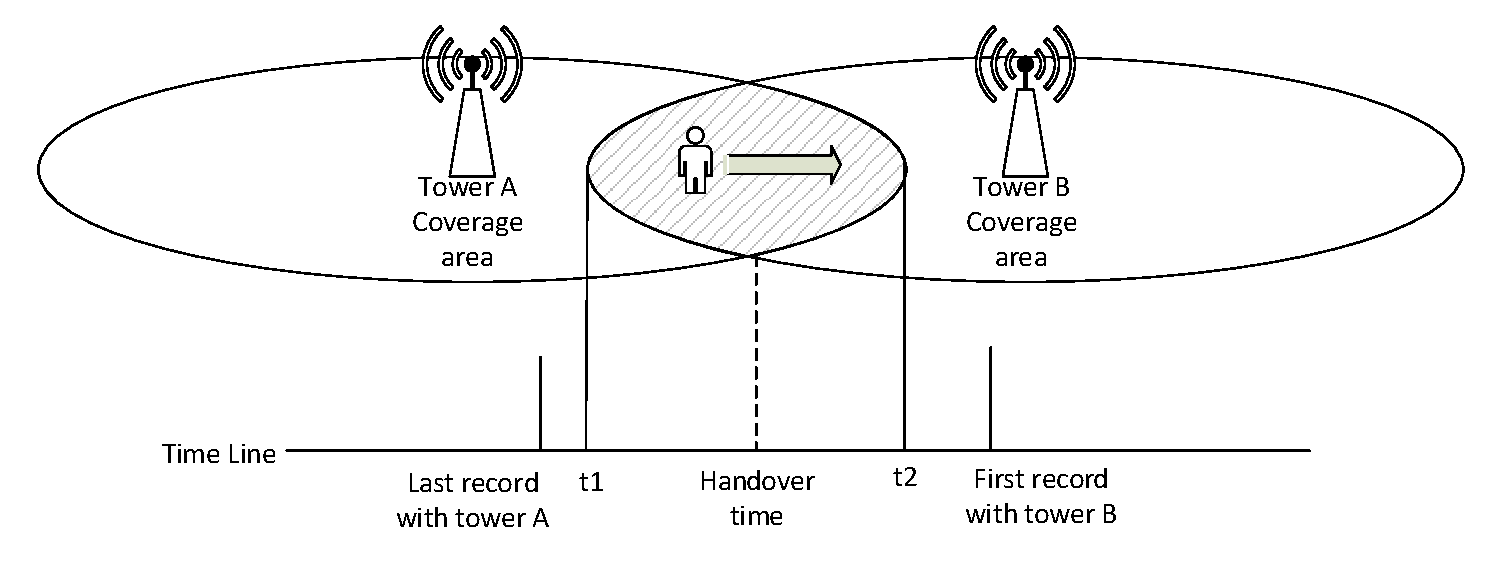
\includegraphics[width=\linewidth]{./figures/passing_boundary.pdf}
    \vspace{-0.3in}
    \caption{A pass-boundary event.}
    \label{fig:pass_bound}
\end{figure}


Formally, a PBE is defined as when a user moving from one tower's coverage cell into an adjacent tower's coverage cell. There are two properties related to a PBE: first, each PBE has a boundary area, which is the overlapping coverage area of two towers; second, each PBE is associated with a time period of the user spent on crossing the boundary area. For example, in \autoref{fig:pass_bound}, the PBE event is associated with a boundary as the shadowed area, while its associated time period is $(t_1, t_2)$ for entering and leaving this shadow area.

We now describe the algorithm on extracting PBEs from the mobile data access traces. For arbitrary two consecutive records $r_i$ and $r_j$ of a user with $l_i$ and $l_j$ as their location estimates respectively, if $l_i \neq l_j$, we define a PBE, denoted by $P_{i, j}$ as follows:
\[
P_{i,j} = (r_i, r_j)
\]
We denote the boundary of $P_{i, j}$, which is the overlapped area, as $(l_i, l_j)$. We use $({t_i}^{last}, {t_j}^{first})$ as an estimate of the time period of entering and leaving $P_{i, j}$, where ${t_i}^{last}$ is the last record timestamp in $l_i$, and ${t_j}^{first}$ is the first record timestamp in $l_j$. The length of the time period of $P_{i, j}$ is bounded by ${t_j}^{first} - {t_i}^{last}$.
Once PBEs are defined, we use them as reference points to decompose mobile data records of each user into segments.

\begin{algorithm}
 \KwData{$Trace$: mobile data trace arranged by users $u$ with record entries $e$ sorted by time. Each $e$ has location estimate $l_e$ and timestamp $t_e$}
 \KwResult{$R$: segments $r$ arranged by user and time.}
 \For{each $u$ in $Trace$}{
	 $l_c \gets \emptyset$,
	 $r \gets \emptyset$,
	 $e_{lastend} \gets \emptyset$,
	 $e_{start} \gets \emptyset$,
	 $e_{end} \gets \emptyset$ \;
	 \For{each $e$ in $Trace[u]$}{
		 \If{$l_c \neq \emptyset$ and $l_c \neq l_e$}{
			 $l_r \gets (l_{e_{lastend}}, l_c, l_e)$,
			 $t_r \gets (t_{e_{start}}, t{e_{end}})$ \;
			 append $r$ to $R[u]$ \;
		 }
		 \If{$l_c = \emptyset$ or $l_c \neq l_e$}{
			 $e_{lastend} \gets e_{end}$,
			 $l_c \gets l_e$,
			 $e_{start} \gets e$
		 }
		 $e_{end} \gets e$ \;
	 }
	 $l_r \gets (l_{e_{lastend}}, l_c, l_e)$,
	 $t_r \gets (t_{e_{start}}, t{e_{end}})$ \;
	 append $r$ to $R[u]$ \;
 }
 \Return{$R$}
 \caption{Data segmentation}\label{alg:Data_segmentation}
\end{algorithm}

The detailed segmentation algorithm is shown in \autoref{alg:Data_segmentation}. Specifically, the decomposition works as follows: we first generate the PBEs for each user, and then we consider all records of a user between two consecutive PBEs as one single stretch of \emph{continuous stay} as such records should be communicating with the same tower. Therefore, they should share the same location estimate. Since we do not have observations on the intra-cell trajectories of user mobility, we consider the user to have the single constant speed for each stretch within a cell, i.e., between two PBE events. To estimate this speed, we use two consecutive PBEs. 
Note, however, that as the first and the last stretches of records only have one PBE each, they will not have speed estimates.

\subsection{Distance and Time Estimation}

We next describe how we estimate the speed between two PBEs. Specifically, we need to estimate the intra-cell boundary-to-boundary distance and the travel time. As the only available information for distance estimation is tower coordinates and tower visiting orders, for a segment with two PBEs $P_{i,j}$ and $P_{j,k}$, we use a straight line trajectory $l_i \rightarrow l_j \rightarrow l_k$ that passes all three tower $l_i$, $l_j$ and $l_k$ as an estimated trajectory. With the coordinates of towers, the euclidean distance between towers, $d(l_i,l_j)$ and $d(l_j,l_k)$, can be calculated. Since the boundaries are perpendicular bisectors of lines connecting towers (as we use Voronoi diagrams to represent cell coverage areas), the travel distance can be estimated by $\frac{d(l_i,l_j) + d(l_j,l_k)}{2}$. Note that if more information such as the underlying road networks are provided, the road trajectories that has the maximum likelihood to match visited tower sequences can also be used instead of the straight line trajectories.

The travel time of a segment is calculated by the time difference of two related PBEs. Since each PBE has a time interval associated with it for entering and leaving the overlapping area, we can calculate a range of possible values for travel time estimation, including both a tight bound and a relaxed bound. The former one suggests the shortest possible travel time to move through the area, while the latter one indicates the longest possible travel time. For example, for two PBEs $P_{i,j}$ and $P_{j,k}$ with a time interval of $({t_i}^{last}, {t_j}^{first})$ and $({t_j}^{last}, {t_k}^{first})$, respectively, we can easily derive the tight bound as $\Delta t_{tight} = {t_j}^{last} - {t_j}^{first}$ and the relaxed bound is $\Delta t_{loose} = {t_k}^{first} - {t_i}^{last}$.

\subsection{Distance Lower Bounds}

In this section, we introduce the concept of distance lower bounds. This is motivated by the observation that it is usually hard to accurately estimate the true distances of users using the coverage areas of given towers for all possible trajectories and represent them with a single distance estimate. To see this, we show an example in \autoref{fig:illustrate_cases}.

\begin{figure}
\centering
\begin{minipage}{.33\textwidth}
  \centering
  {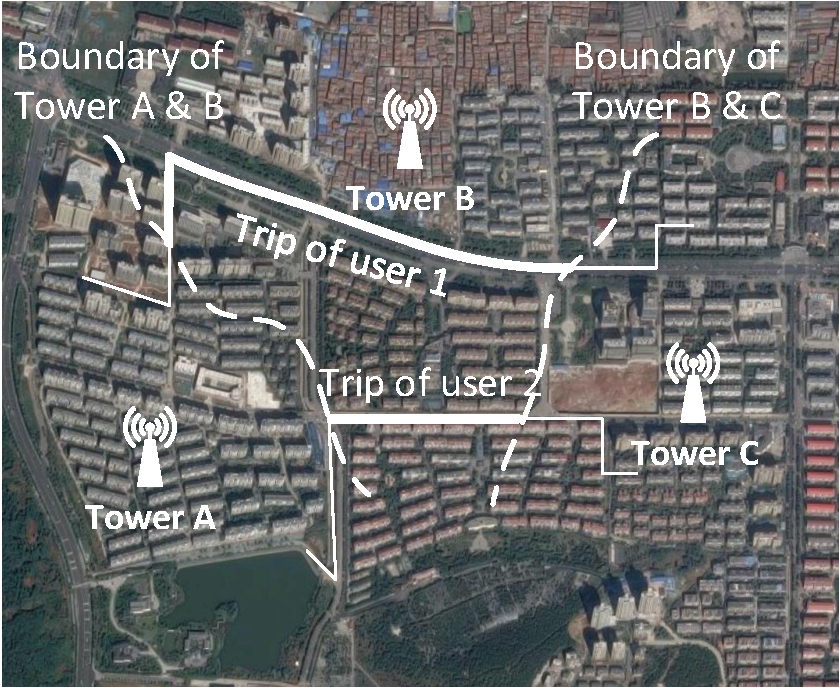
\includegraphics[width=0.944\linewidth]{./figures/illustrate_cases.pdf}}
  \captionof{figure}{Common cases where a single \newline distance estimate would fail}
  \label{fig:illustrate_cases}
\end{minipage}%
\begin{minipage}{.33\textwidth}
  \centering
  {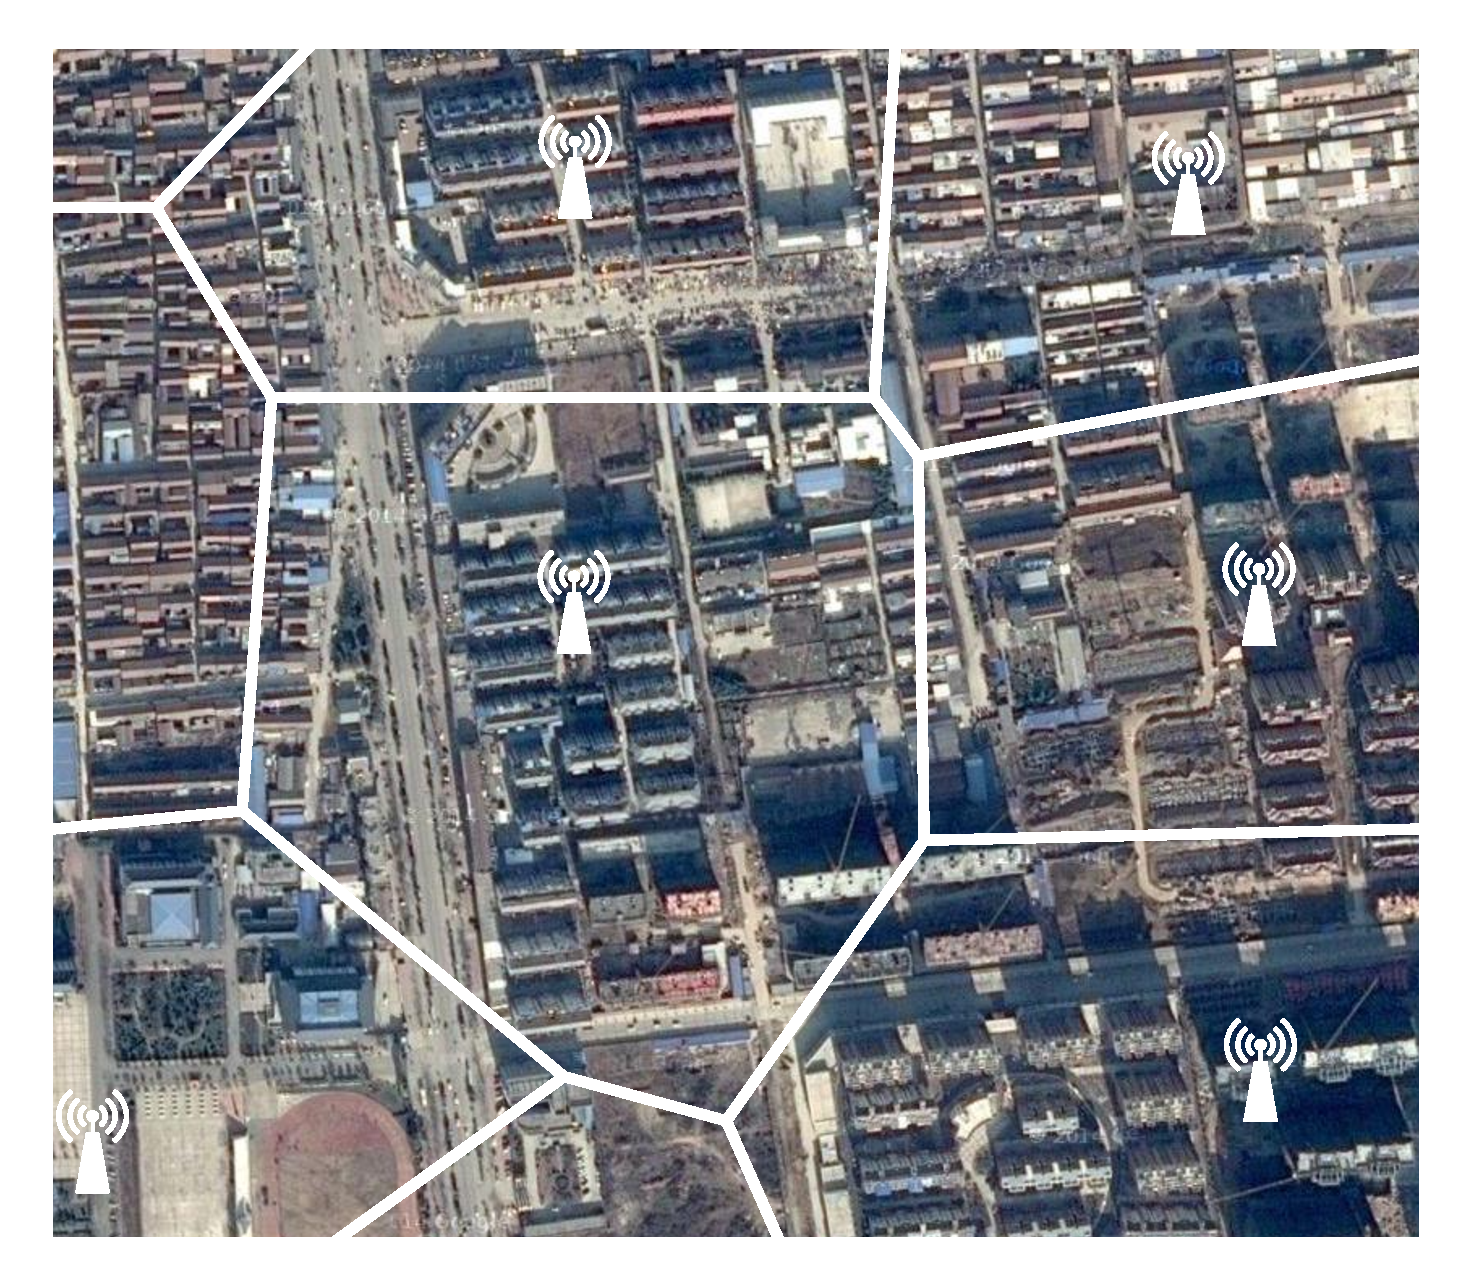
\includegraphics[width=0.9\linewidth]{./figures/voronoi_illustrate.pdf}}
  \captionof{figure}{Voronoi diagram to represent \newline communication coverage of each tower}
  \label{fig:voronoi}
\end{minipage}
\begin{minipage}{.33\textwidth}
  \centering
  \vspace{0.1in}
  {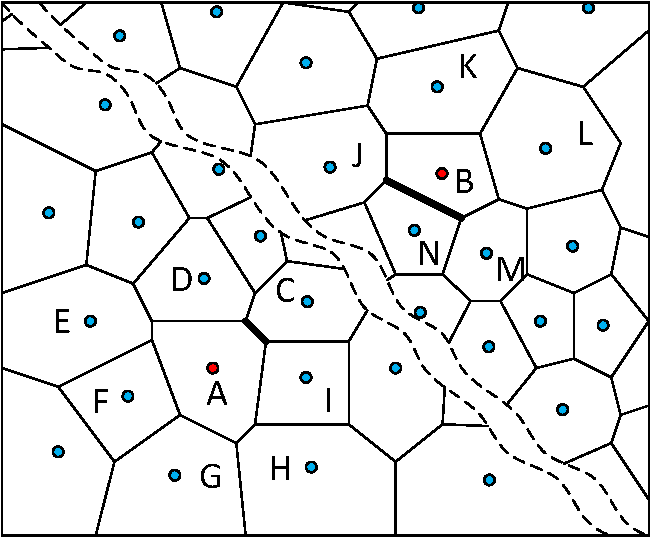
\includegraphics[width=0.935\linewidth]{./figures/virtual_boundary.pdf}}
  \captionof{figure}{Dealing with virtual boundaries}
  \vspace{0.25in}
  \label{fig:virtual}
\end{minipage}
\end{figure}

% \begin{figure}[h]
%     \centering
%     \vspace{-0.1in}
%     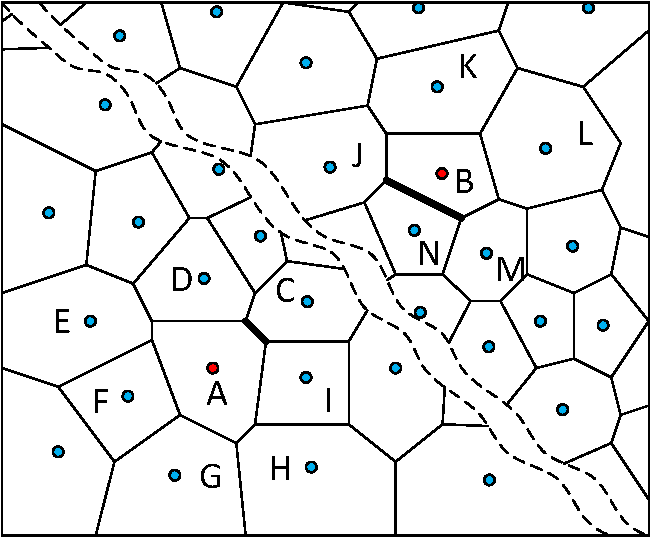
\includegraphics[width=0.9\linewidth]{./figures/virtual_boundary.pdf}
%     \vspace{-0.2in}
%     \caption{Dealing with virtual boundaries.}
% 		\label{fig:virtual}
% \end{figure}


% \begin{figure}[h]
%     \centering
%     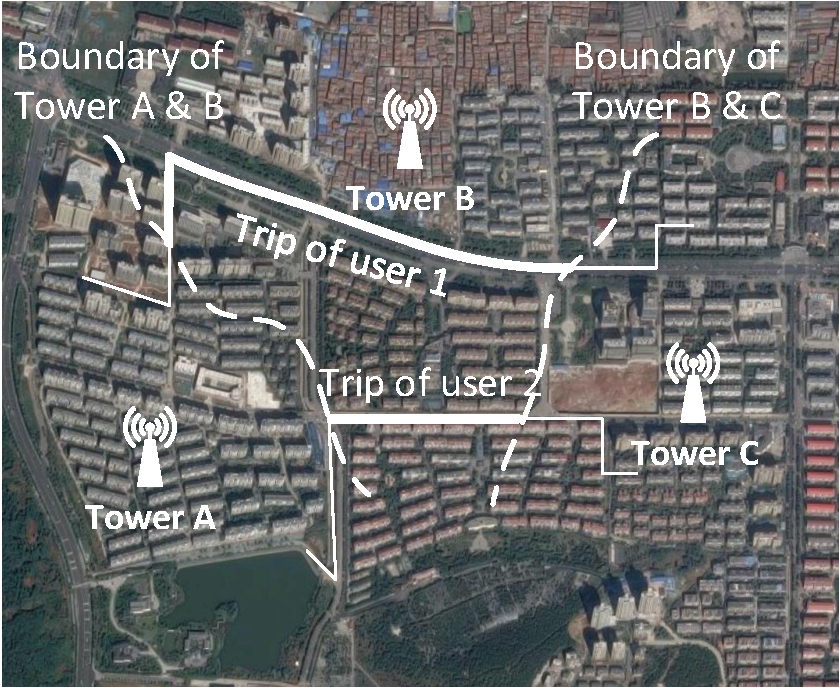
\includegraphics[width=\linewidth]{./figures/illustrate_cases.pdf}
%     \vspace{-0.4in}
%     \caption{Common cases where a single distance estimate would fail.}
%     \label{fig:illustrate_cases}
%     \vspace{-0.1in}
% \end{figure}


As shown in \autoref{fig:illustrate_cases}, the area is divided into coverage areas of three towers $A$, $B$, and $C$. Solid lines represent real user trajectories while dashed lines represent the boundaries of towers. Observe that both user $1$ and user $2$ pass the three towers in the same order $A - B - C$. The real distance differences, however, are missing due to the limited location estimation accuracy of using tower locations. Therefore, in such cases, a single distance estimate will have to fail due to the wide variety of possible trajectories that can lead to the same tower visiting orders.

Faced with this challenge, our next goal is to filter out distance estimates that are not likely to occur in real world scenarios, and provide the trajectory that is most likely as the solution. The major step here is to evaluate the confidence levels of different distance estimates based on estimated trajectories and tower locations so that such confidence levels can be used as measures for evaluating differences in multiple trajectory lengths. Specifically, for two consecutive boundary events $P_{i,j}$ and $P_{j,k}$, the confidence level of a distance estimate $d_{est}$ is defined as $C_{d_{est}} = \frac{d_{lb}}{d_{est}}$, where $d_{lb}$ is the boundary-to-boundary distance lower bound, i.e., the minimum required distance to travel from the boundary of $P_{i,j}$ to the boundary of $P_{j,k}$, which serves as a conservative estimate for the shortest distance a user may travel. Intuitively, the longer an estimated distance is compared to this lower bound, the less likely it should be as it requires a more complex trajectory shape to be feasible.

% \begin{figure}[h]
%     \centering
%     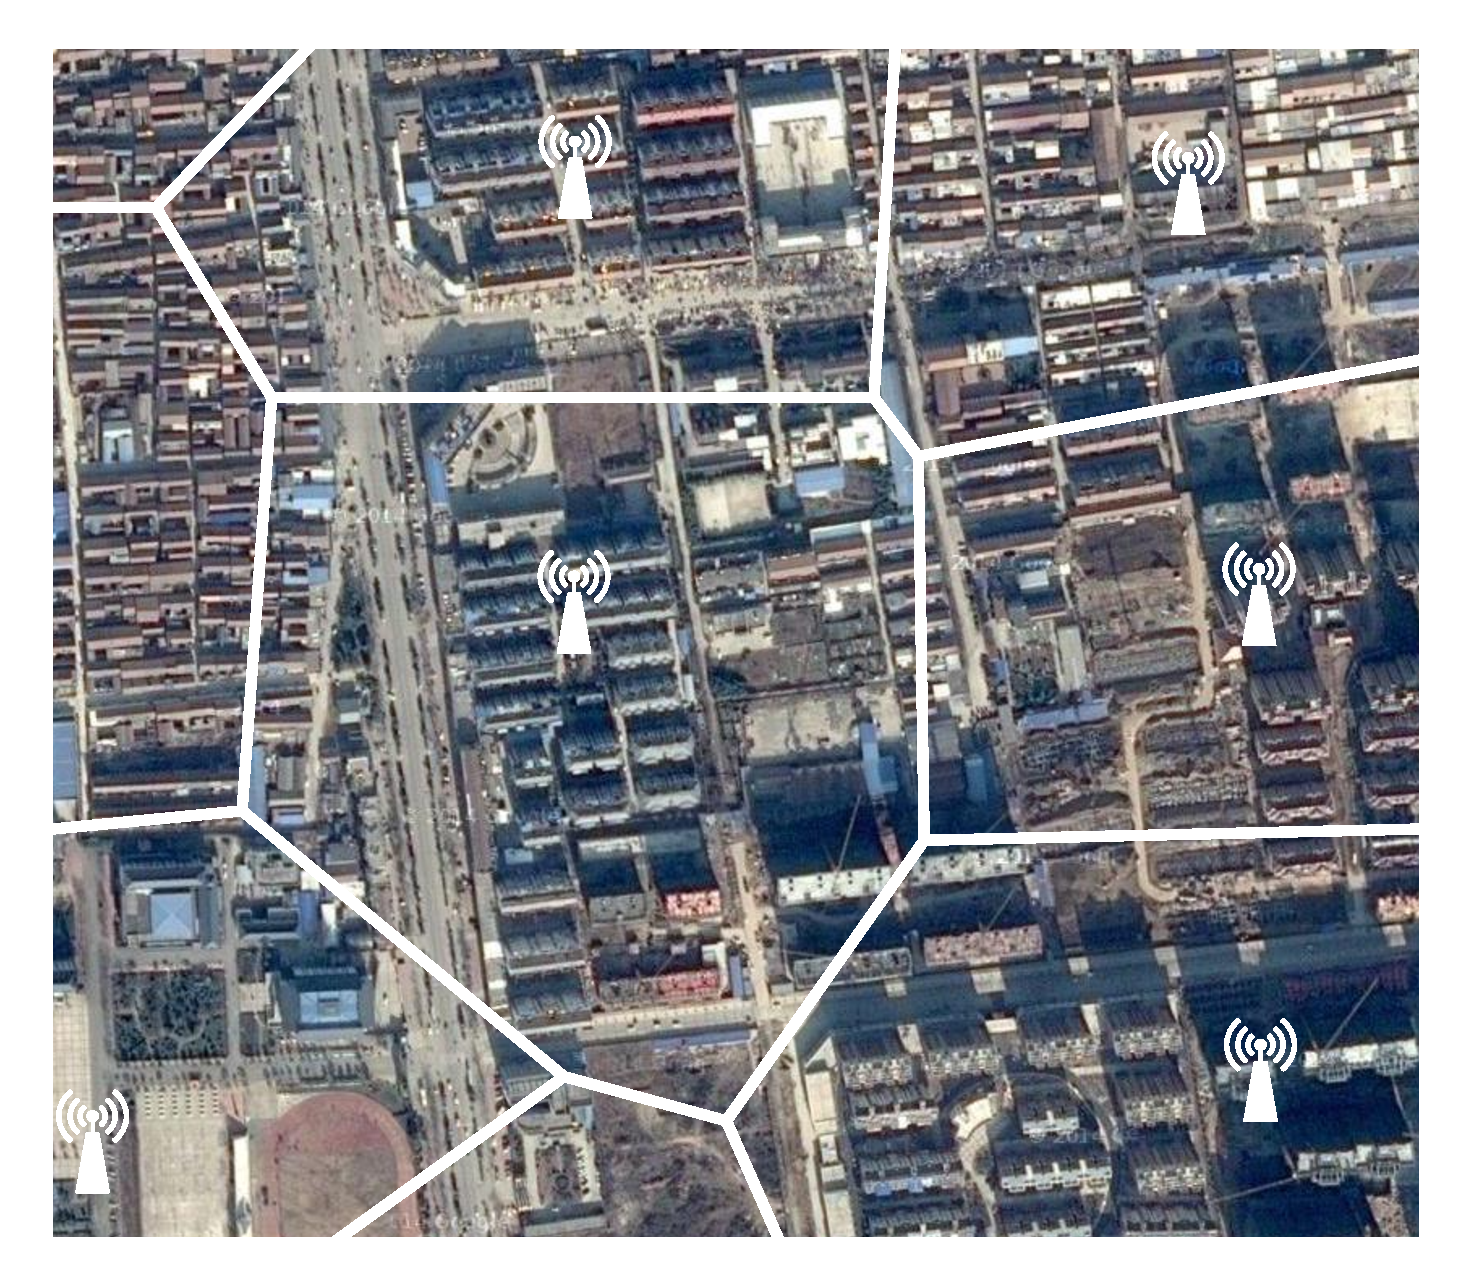
\includegraphics[width=0.9\linewidth]{./figures/voronoi_illustrate.pdf}
%     \vspace{-0.1in}
%     \caption{Voronoi diagram to represent communication coverage of each tower.}
% 		\label{fig:voronoi}
%     %\vspace{-0.1in}
% \end{figure}

In order to calculate the distance lower bound, 
we first simplify the tower coverage model with the Voronoi diagram. 
%the assumption that 
%cell phones only communicate with the nearest tower, 
%and towers have same transmission power. 
Then, based on the Voronoi diagram formed by towers' locations, we calculate the Voronoi cell shapes with their vertex locations. 
\autoref{fig:voronoi} shows an example of the Voronoi diagram construction with five towers. 
Each region in the Voronoi diagram represents the coverage area of one tower, while the edges in Voronoi diagrams are central focus lines of overlapping coverage area of towers (such areas are hidden in simple Voroni diagrams, but they widely exist in real-world tower communications).  
The shortest travel distance between boundaries is therefore transformed into the shortest distance between two Voronoi edges, 
and can be solved using simple geometric methods. The detailed algorithm is shown in \autoref{alg:DLB_estimation}.

\begin{algorithm}
 \SetKwComment{comment}{//}{}
 \KwData{$TC$: a list of tower coordinates.}
 \KwResult{$D_{lb}$: a list of all boundary-to-boundary distance lower bounds estimated from Voronoi diagram.}
 %\comment{project to euclidean space with equirectangular projection}
 $TL \leftarrow TC$; $P \leftarrow TL$ \;
 Build Voronoi diagram $VD$ with $P$ \;
 \For{each $edge1$ in $VD$}{
	 $pset1 \gets$ Voronoi points of $edge1$ \;
	 \For{each $edge2$ in $VD$}{
		 $pset2 \gets$ Voronoi points of $edge2$ \;
		 \If{$pset1 \cap pset2 \neq \emptyset$}{
			 $D_{lb}[(pset1, pset2)] \gets |edge1 - edge2|$\;
		 }
	 }
 }
 \Return{$R$}
 \caption{Distance lower bound estimation}\label{alg:DLB_estimation}
\end{algorithm}

%If we have an estimated distance that is much longer than the distance lower bound, then the possibility that there are trajectories of large distance differences connecting two boundaries is high. Therefore, the confidence level of using the distance estimate to represent the distance of all possible trajectories is low. On the contrary, if the estimated distance is very close to the distance lower bound, then the confidence level of estimated distance is high and the distance estimate should be able to represent the length of most trajectories between two boundaries.

\subsection{Virtual Boundaries}

A fundamental limitation of using cellphone-tower communication datasets is that records are only collected when mobile data accesses are happening. If the user is keeping silent, there is no way for us to know their locations. In such cases, if the user has traveled across multiple boundaries, we may encounter the following observation: we analyze the consecutive records for this user and find out that their $l_i$ and $l_j$  may be far away from each other and do not necessarily share a common boundary area. If $l_i$ and $l_j$ are adjacent to each other, we say to $P_{i,j}$ has a real boundary. Otherwise, we refer to it as a virtual boundary.

Different from real boundaries that are treated as an edge in the Voronoi diagram, virtual boundaries are actually distance estimates themselves as users have passed the coverage area of several towers during a PBE within a virtual boundary. Since we do not have any information regarding which towers the user has visited in between, to calculate the distance lower bound of a virtual boundary, we instead use the shortest distance of all possible boundary pairs of $l_i$ and $l_j$ as the best estimate.

We now give an example in \autoref{fig:virtual}, where we analyze two consecutive records: $r_i$ for tower $A$ and $r_j$ for tower $B$. Since tower $A$ and tower $B$ do not share physical boundaries, they only have a virtual boundary between them. To calculate their shortest distance, we calculate the distance from each boundary of tower $A$ to each boundary of tower $B$ and use the shortest one of all boundary pairs as the estimated distance. In this example, the distance between boundary $(A, C)$ and boundary $(B, N)$ is used as the distance lower bound of the virtual boundary $(A, B)$.

% \begin{figure}[h]
%     \centering
%     \vspace{-0.1in}
%     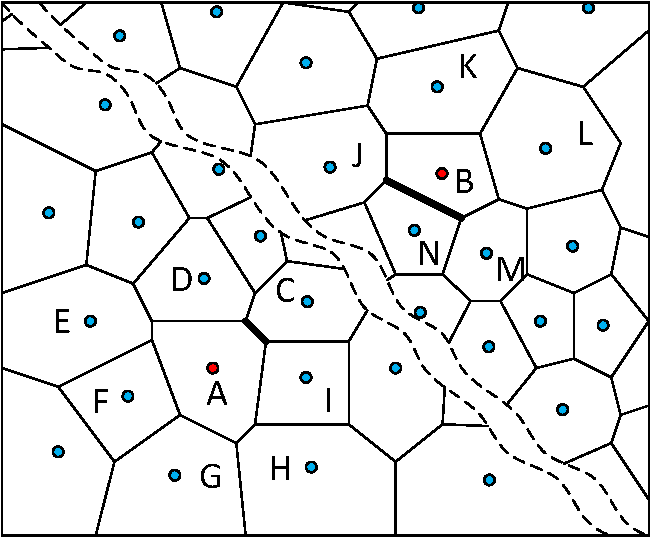
\includegraphics[width=0.9\linewidth]{./figures/virtual_boundary.pdf}
%     \vspace{-0.2in}
%     \caption{Dealing with virtual boundaries.}
% 		\label{fig:virtual}
% \end{figure}

Returning to our earlier analysis, for segments that have PBEs with virtual boundaries, we merge them with adjacent segments if they exist. The distance estimate and lower bound of a segment are the sum of distance estimates and distance lower bounds of both records, and if any, the virtual boundaries between them. Note that as we calculate the sum of distance lower bounds, the resulting distance lower bound is still the minimum distance required to reach one real boundary from the other, even this requires that the trajectory should pass through virtual boundaries  between consecutively visited towers.

\subsection{Speed Estimation}

Now that we have a distance estimate $d_{est}$, a distance lower bound $d_{lb}$, and a range of possible travel time represented as $(\Delta t_{tight}, \Delta t_{loose})$ for each segment, we can infer the travel time of a segment estimated by $\Delta t_{est} = \frac{\Delta t_{tight} + \Delta t_{loose}}{2}$. We denote this by $\Delta t_{est}$. We next calculate the confidence levels for both distance estimates and travel time estimates as follows:
\begin{eqnarray}
  C_{d_{est}} &=& \frac{d_{lb}}{d_{est}} \\
  C_{\Delta t_{est}} &=& \frac{\Delta t_{est}}{\Delta t_{loose}}
\end{eqnarray}

By setting a threshold for both confidence levels, we can filter out estimates that are not accurate enough. Although we can filter out more inaccurate speed estimates with a much stricter threshold in both confidence levels, we may end up with a limited number of records that have qualified speed estimates. Finally, after setting proper threshold for confidence levels, the speed of the user can be estimated as the following:
\begin{equation}
  s_{est} = \frac{d_{est}}{\Delta t_{est}}
\end{equation}
The detail of the speed estimation algorithm is shown in \autoref{alg:speed_est}.


\begin{algorithm}
 \SetKwComment{comment}{//}{}
 \SetKwInput{KwParam}{Param}
 \KwData{$R$ from \autoref{alg:Data_segmentation} and
 %: mobile data records arranged by segments $r$;
%					$r$: A mobile data segment which has:
%					$l_{pre}, l, l{post}$: location estimates for segment before $r$, itself and segment after $r$, where $l_{pre}$ and $l_{post}$ are acquired during BPE extraction;
%					$d_{est}$:distance estimates;
%					($\Delta t_{tight}$, $\Delta t_{loose}$): travel time estimates;
          $D_{lb}$ from \autoref{alg:DLB_estimation}. %: a list of boundary-to-boundary distance lower bound estimated from Voronoi diagram.
          }
 \KwParam{$T_{C_{d}}$, $T_{C_{t}}$: confidence level threshold for distance estimates and travel time estimates.}
 \KwResult{$S$: Speed estimates for each segment.}
 \For{each $r$ in $R$}{
	 \comment{Check if $r$ has real boundary and find its distance lower bound}
	 \eIf{$((l_{pre}, l), (l, l_{post}))$ is not in $D_{lb}$}{
		 combine $r$ with next record \;
		 continue \;
	 }
	 {
		 $d_{lb} \gets D_{lb}[(l_{pre}, l), (l, l_{post})]$ \;
	 }
	 \comment{Calculate travel time estimates}
	 $\Delta t_{est} \gets \frac{\Delta t_{tight} + \Delta t_{loose}}{2}$ \;
	 \comment{Calculate confidence level}
	 $C{d_{est}} \gets \frac{d_{lb}}{d_{est}}$ ;
	 $C_{\Delta t_{est}} \gets \frac{\Delta t_{est}}{\Delta t_{loose}}$ \;
	 \comment{Estimate speed if meet threshold}
	 \If{$C{d_{est}} \geq T_{C_{d}}$ and $C_{\Delta t_{est}} \geq T_{C_{t}}$}{
		 $s_{est} \gets \frac{d_{est}}{\Delta t_{est}}$ ;
		 $S[r] \gets s_{est}$ \;
	 }
 }
 \Return{$S$}
 \caption{Speed estimation}\label{alg:speed_est}
\end{algorithm}


\subsection{Cell Oscillation and Speed Compensation}

The distance lower bounds can also help to eliminate the cell oscillation problem, i.e., when a user near boundary area randomly communicates with two or more towers in short periods, generating a sequence of false pass-boundary events. Since the user keeps passing the same boundary, the distance lower bound for such scenarios should always be $0$. Therefore, the confidence level of distance estimates will also be $0$, which means that we can detect them and filter them out.

Since segments between these false PBEs usually have very short durations due to the nature of how they are generated, we estimate the speed for such segments based on the assumption that a user's speed does not change dramatically in a very short time period. Therefore, for a segment between false PBEs, if there is a segment that happens to be very close to it and has a qualified speed estimate,  we will use its speed estimate as the speed estimate for the segment with false PBEs. Other kinds of low confident level speed estimations can also be compensated by the nearby segments with high confidence levels as long as the confidence level and time period are properly handled.


\section{Experimental Results}\label{experiments}

With our methodology on speed estimates, we next explain our findings on correlations between user mobility and mobile data access patterns in this section. We start with the correlation of the speed and the average mobile data access volumes. Then we reveal the relation of speed and average time intervals between consecutive mobile data accesses. Finally, we illustrate the correlation between speed and the types of app usage that are responsible for generating the corresponding mobile data traffic.

\begin{figure}[h]
    \centering
    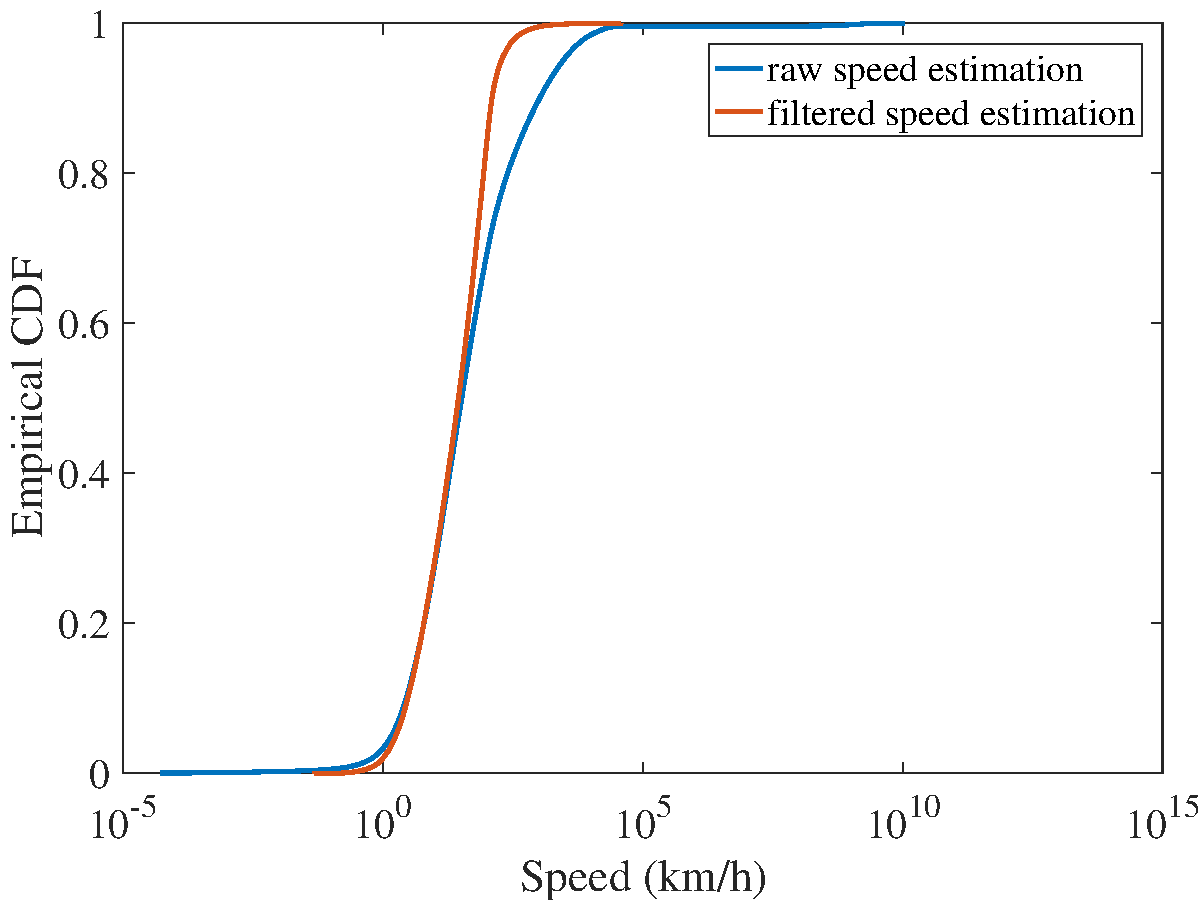
\includegraphics[width=0.5\linewidth]{./figures/speed_cdf.pdf}
    \caption{Empirical CDF of speed estimates.}
    \label{fig:speed_cdf}
\end{figure}

\subsection{Experiment Settings}

To estimate the speed, our algorithm requires a user has visited at least 3 towers consecutively. In the dataset, we find that around 13 million records out of 58 million records can be utilized. Although the dataset contains both user initiated network access and background network access, we find it very hard to separate them reliably. In our experiments, to balance the accuracy of speed estimates and the number of mobile data access records that have qualified speed estimates, we set the threshold of both distance ratio $d_{ratio}$ and duration ratio $\Delta t_{ratio}$ empirically as 0.6. After the filtering, we have around 1 million records out of total 13 million records that meet both criteria. \autoref{fig:speed_cdf} shows the cumulative density function (CDF) of both raw speed estimates without filtering and filtered speed estimates. As we can see that the filtered speed estimates are more realistic compared to raw speed estimates. Most of the false high speed estimates and low speed estimates are filtered out by setting thresholds of confidence levels for distance estimates and travel time estimates.

In the following experiments, we only show results in the speed range from 0 km/h to 100 km/h, since there are very few records with a speed estimate above 100 km/h for any meaningful insights.

\subsection{Speed and Data Volumes}

\begin{figure*}
    \centering
		\subfigure[Data Volume\label{fig:speed_vol}]{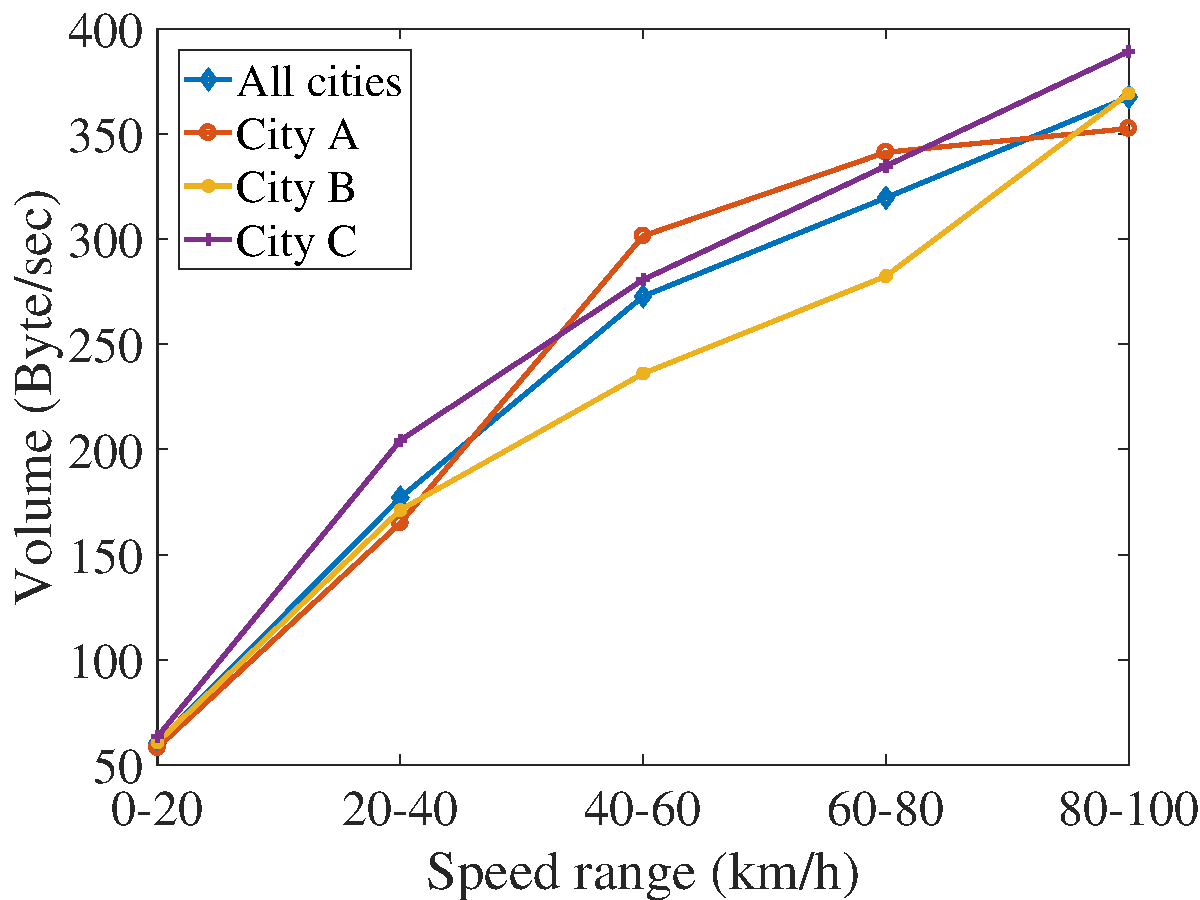
\includegraphics[width=0.48\linewidth]{./figures/large_font/speed_vol.pdf}}
    \subfigure[Average Time Interval\label{fig:speed_gap}]{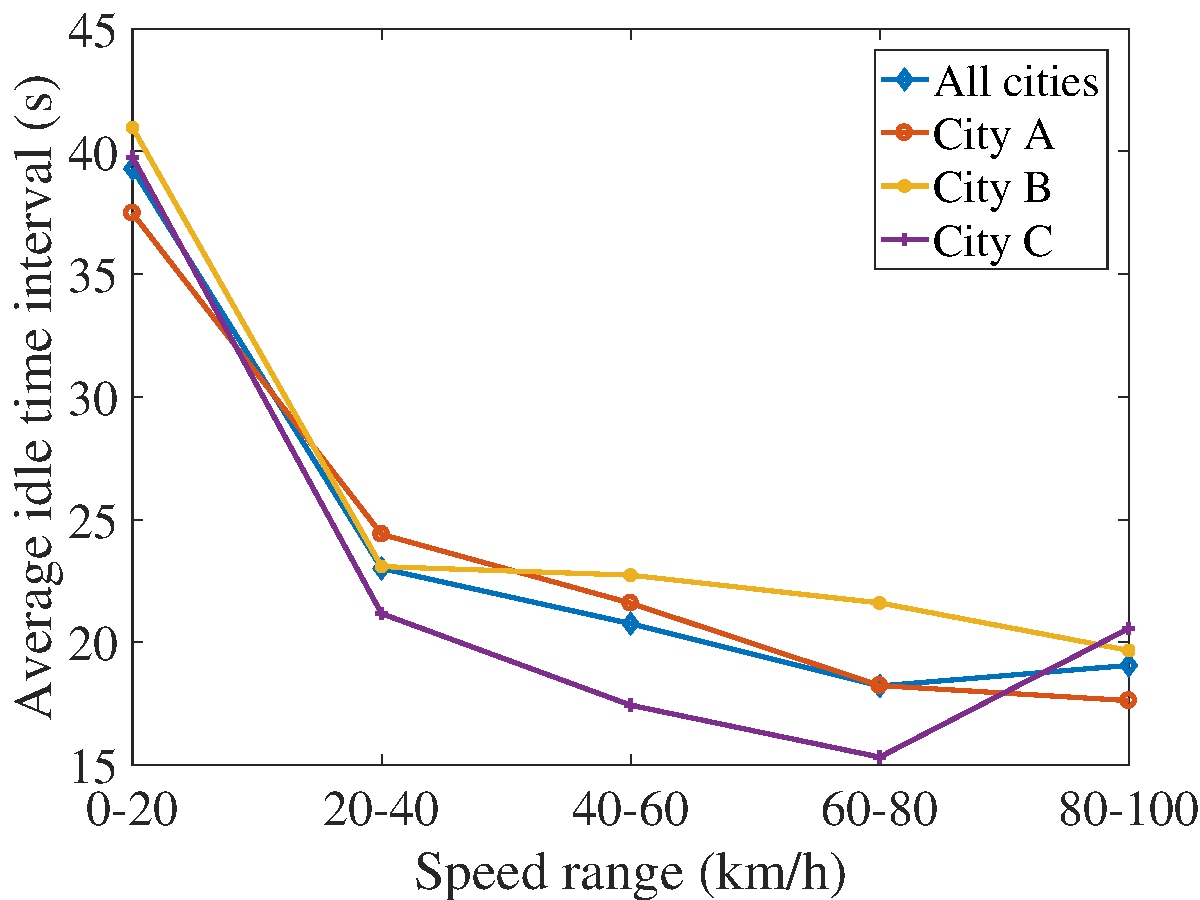
\includegraphics[width=0.48\linewidth]{./figures/large_font/speed_gap.pdf}}
		\subfigure[Time Interval Empirical CDF\label{fig:speed_gap_cdf}]{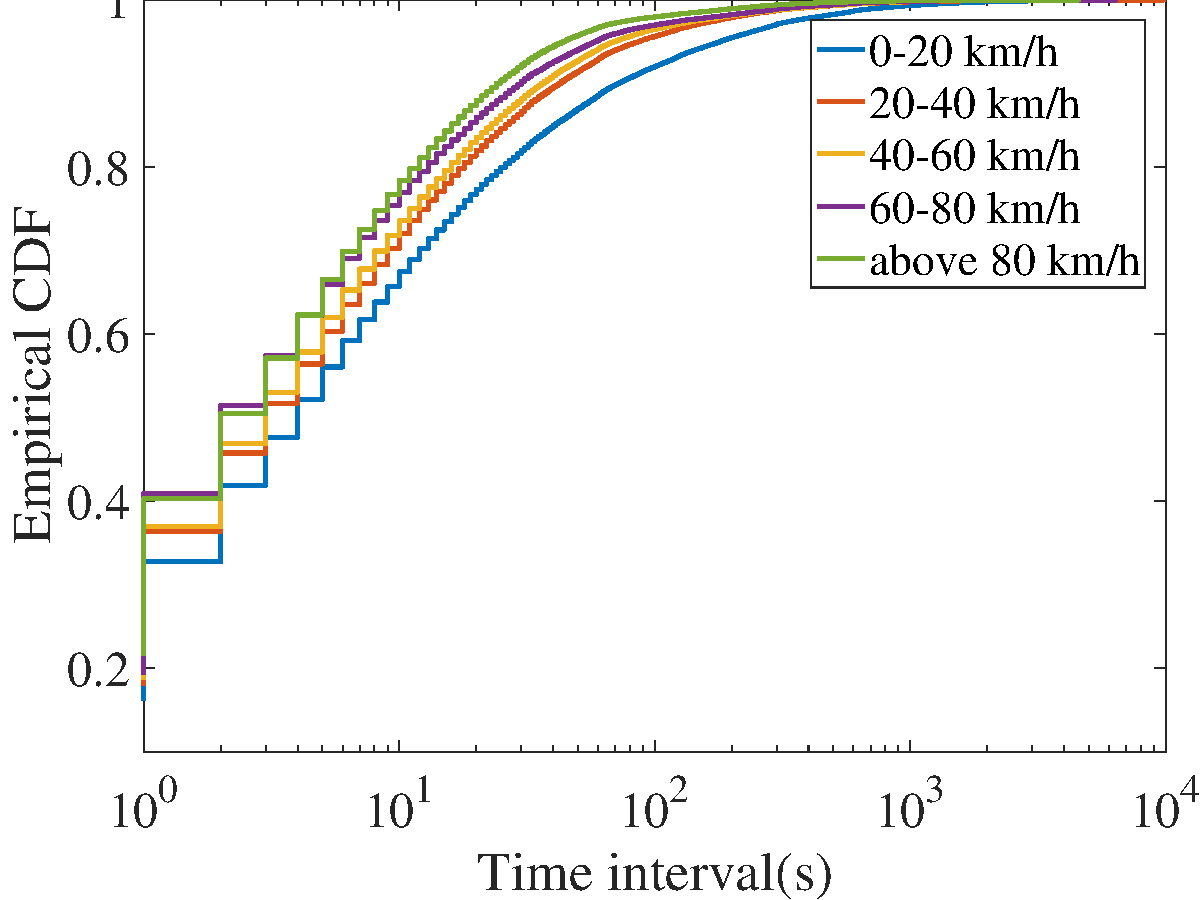
\includegraphics[width=0.48\linewidth]{./figures/large_font/speed_gap_cdf.pdf}}
		\subfigure[Average Volume per Data Access\label{fig:speed_per_conn_vol}]{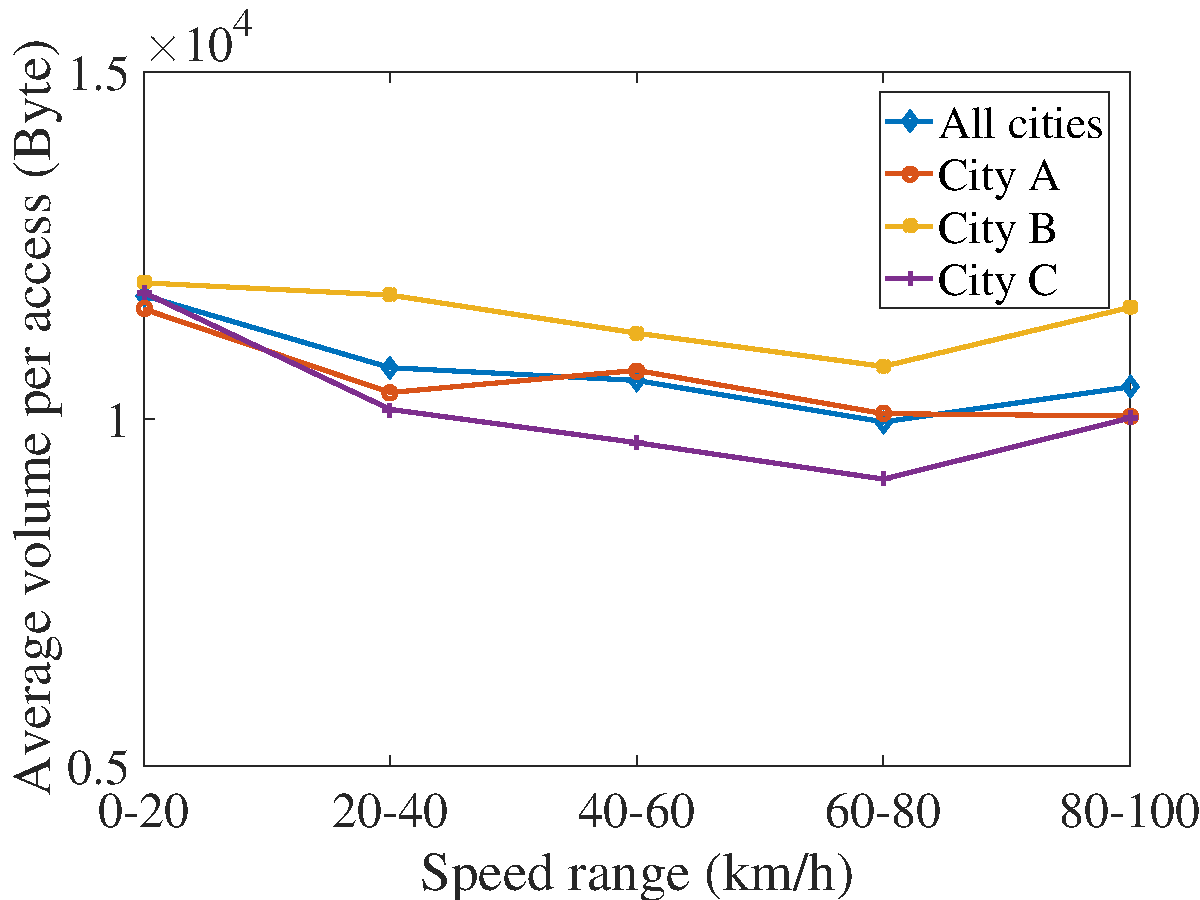
\includegraphics[width=0.48\linewidth]{./figures/large_font/speed_per_conn_vol.pdf}}
    \caption{The correlation of speed estimates with (a) data volume, (b) average idle time interval between consecutive data access, (c) idle time interval between consecutive connections, (d) average data access volume for each data access.}
    \label{fig:speed_corr}
\end{figure*}

\autoref{fig:speed_vol} shows the results of the correlation of user speed and the average mobile data access volumes per user per second. We demonstrate the data from all three cities combined and each city respectively. The figure shows a clear trend that users are more active in accessing mobile data as the speed increases and the trend holds true for all three cities. In fact, a user with speed estimates of 80-100 km/h could reach an average data volume of 6 times of a low-speed user. Similarly, this trend also holds true for all the cities. Note that these results only show an increase in the mobile data access volume as user speed increases. It does not suggest lower speed users access online contents less frequently. Actually, we believe one reason might be that a large portion of a low-speed user's online needs is already fulfilled by various kind of high-speed connections such as Wifi hotspots. To this end, we reach similar findings with previous work~\cite{yang2015characterizing} on the correlation of user mobility and mobile data access volume, except that the previous work used the number of towers visited by a user as the indicator of user mobility.

\subsection{Speed and Access Frequency}

\autoref{fig:speed_gap} shows the correlation of speed and average idle time intervals between consecutive mobile data access records. The CDF of data time intervals for various speed ranges of all three cities are also shown in \autoref{fig:speed_gap_cdf}. Note that since the time precision of our data trace is seconds, so there are steps in \autoref{fig:speed_gap_cdf}. The decrease in time intervals as speed increases suggests that high-speed user accesses mobile data more frequently than low-speed users. A user with a speed estimate of 80-100 km/h access mobile data almost twice more frequently than a user with a speed estimate of 0-20 km/h on average. The trend holds for all three cities except that there is an odd point at 80-100 km/h for one city, which may be caused by the lacking of available data.

We show the average volume for each data access in \autoref{fig:speed_per_conn_vol}. As the user speed increases, there is no apparent correlation with average volume for each data access. This suggests that increasing in the average volume which is shown in \autoref{fig:speed_vol} is mainly cause by the increased data access frequency, not the volume for each data access.

\subsection{Speed and App Usage}

According to the mobile service provider, each app in our dataset was assigned to one of 18 categories, as shown in \autoref{table:appcat}.
\begin{table}[h]
	\centering
	\begin{tabular}{lrr}\hline
	App Category & \# Apps & Volume (GB) \\
    \hline
	Instant Messages & 30 & 97.3\\
	Reading & 101 & 17.6\\
	Microblog & 43 & 13.0\\
	Navigation  & 38 & 10.8\\
	Video  & 63 & 45.2\\
	Music  & 33 & 27.4\\
	App Market & 45 & 37.0\\
	Game  & 106 & 9.2\\
	Payment & 18 & 1.2\\
	Comic & 12 & 0.8\\
	Email & 10 & 1.5\\
	P2P & 8 & 3.9\\
	VOIP  & 17 & 0.3\\
	Multimedia Messages & 2 & 0.3\\
	Browsing & 558 & 353.5\\
	Finance  & 25 & 0.7\\
	Security  & 22 & 5.2\\
    Others  & 244 & 95.8\\
% 	Other1 & 237 & 74.7\\
% 	Other2 &   7 & 21.1\\
% 	Others & 464 & 118.9\\
    \hline
	\end{tabular}
	\caption{App categories}
	\label{table:appcat}
\end{table}

\begin{figure}[h]
    \centering
    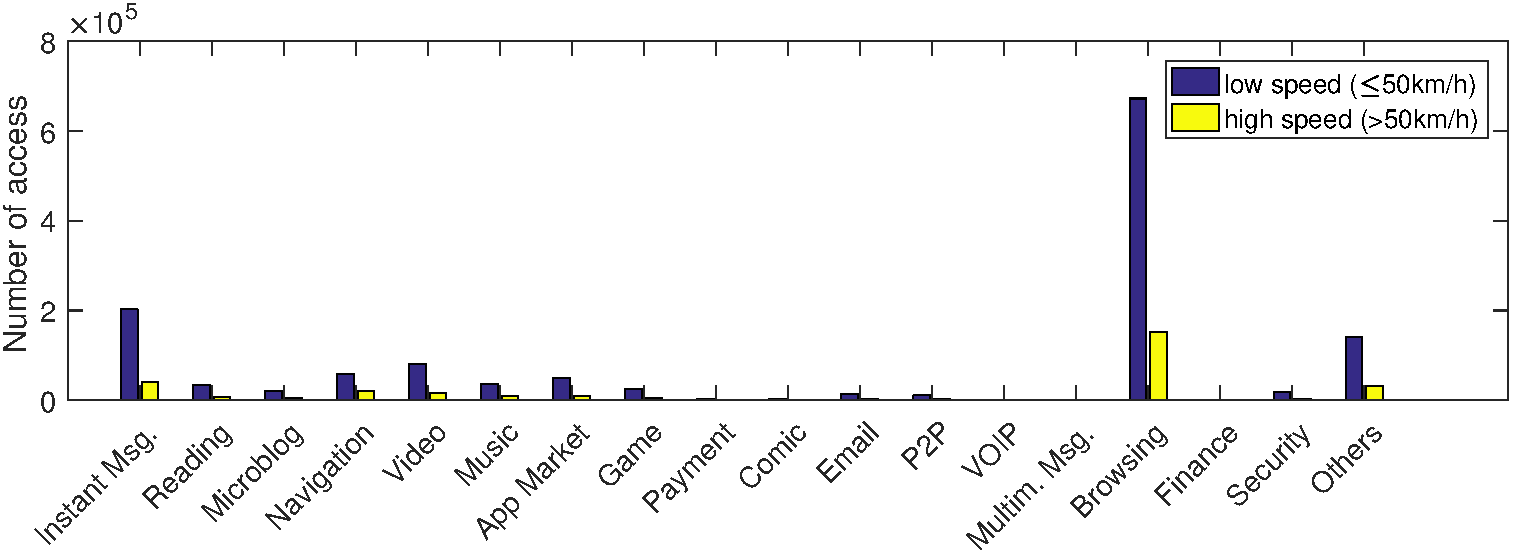
\includegraphics[width=\linewidth]{./figures/num_access_high_low_speed_8_6.pdf}
    \caption{The distribution of the number of access per app category with high and low speed users}
    \label{fig:speed_access_hl}
\end{figure}

\begin{figure}[h]
    \centering
    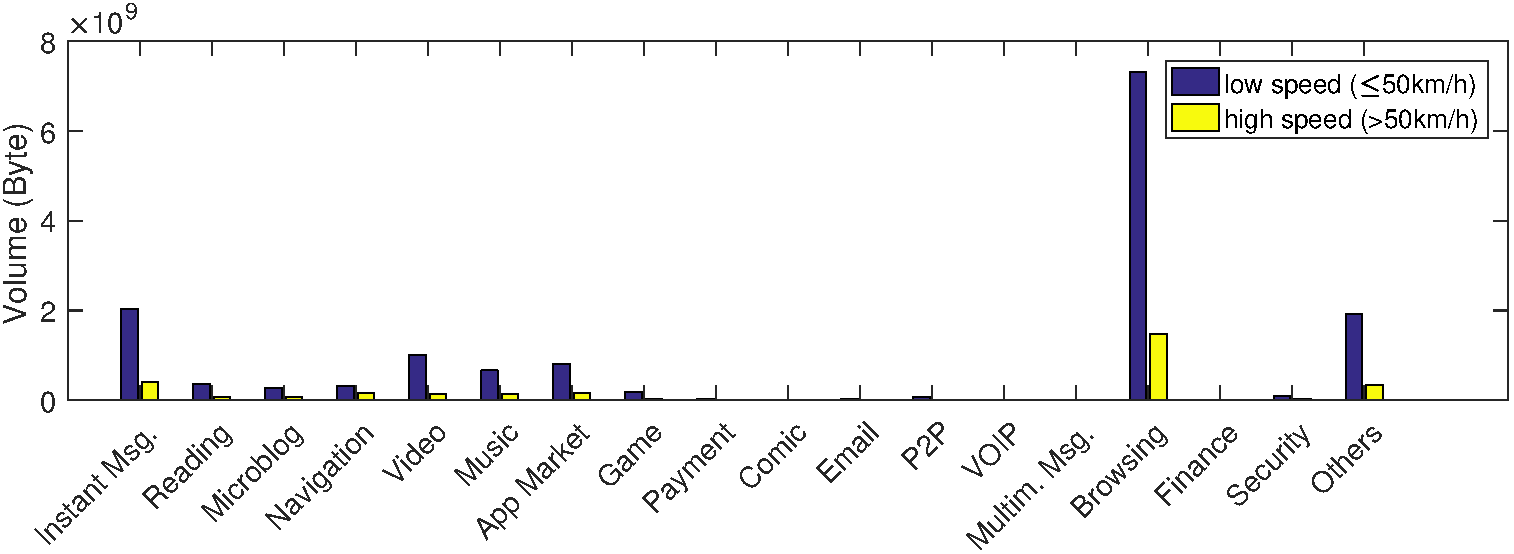
\includegraphics[width=\linewidth]{./figures/volume_high_low_speed_8_6.pdf}
    \caption{The distribution of data volume per app category with high and low speed users}
    \label{fig:speed_vol_hl}
\end{figure}

We first divided the estimated user speed by 50km/h into two classes. The low speed class includes transportation modes such as walking, cycling, bus and other low speed vehicles. The high speed class includes mainly high speed vehicles. We showed the number of data access per app category in \autoref{fig:speed_access_hl} and data volume per app category in \autoref{fig:speed_vol_hl}. In both figures, low speed users have more data access due to large user base. The share for each category holds similar trend for both high and low speed users. We will discuss more details on the contribution of each category to total data access in \autoref{fig:speed_appcat}.

\begin{figure*}
    \centering
		\subfigure[Number of unique apps used per minute\label{fig:app_per_min}]{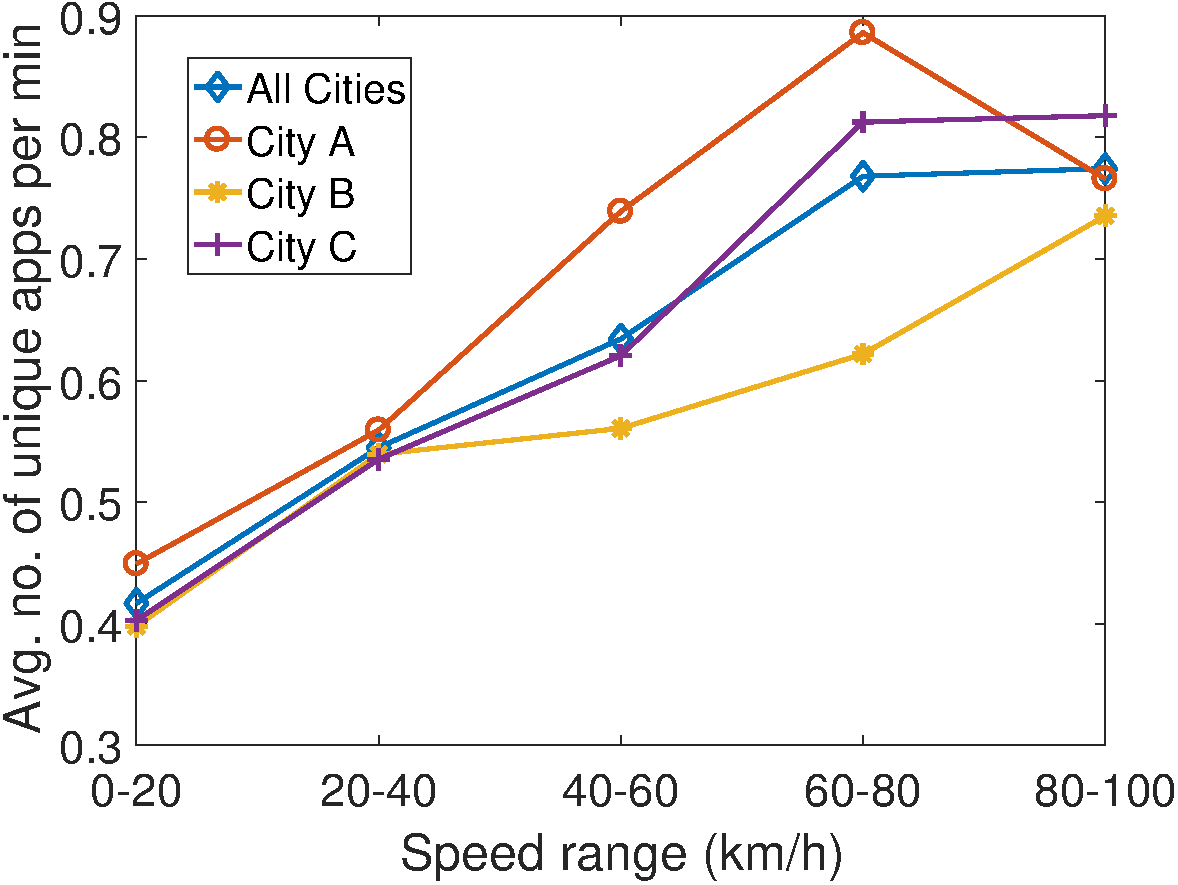
\includegraphics[width=0.48\linewidth]{./figures/app_per_min_8_6.pdf}}
		\subfigure[Number of unique app categories used per minute\label{fig:app_cate_per_min}]{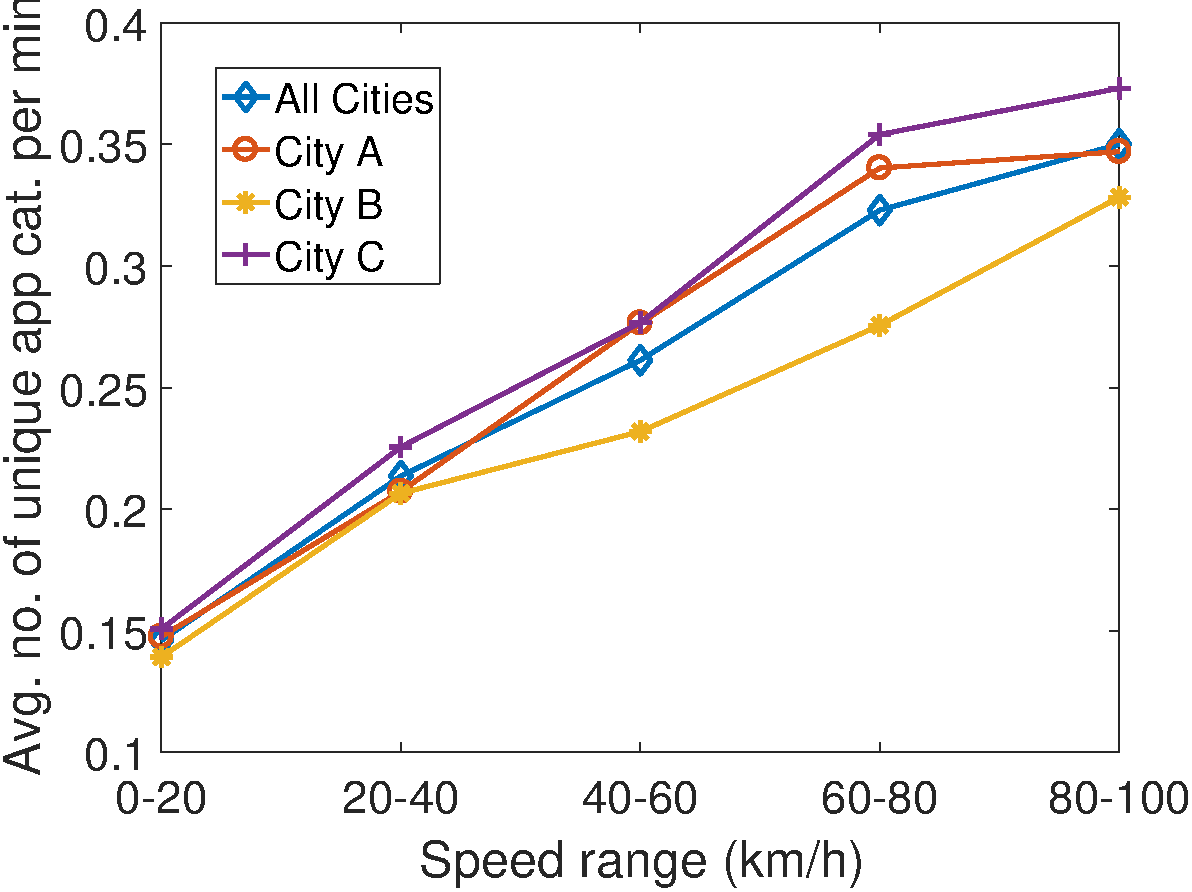
\includegraphics[width=0.48\linewidth]{./figures/app_category_per_min_8_6.pdf}}
    \caption{Correlation of user speed and the number of unique apps and app categories used}
    \label{fig:speed_app_used}
\end{figure*}

%In this section, we first show in
\autoref{fig:speed_app_used} shows the correlation between user speed and the average number of unique apps and app categories being used for each user during each data segment per minute.
The trend clearly shows that as the speed goes up, the app usage diversity increases rapidly.
A user with a speed estimate of 80-100 km/h could use as many as 2 times apps per unit of time compared to a low-speed user.
% This trend holds true for all the cities. 
An explanation might be that for users with high mobility, they may use their phones more often, use more kinds of apps, and be less likely to focus on one app for prolonged periods of time. 
% Both \autoref{fig:speed_app_used} and \autoref{fig:speed_app_switch} lead to the similar conclusion that unlike low speed users, users with high mobility may use their phones more often, switch between apps more, and be less likely to focus on one app for prolonged periods of time. 

\begin{figure*}
    \centering
		\subfigure[App switch frequency\label{fig:switch_app}]{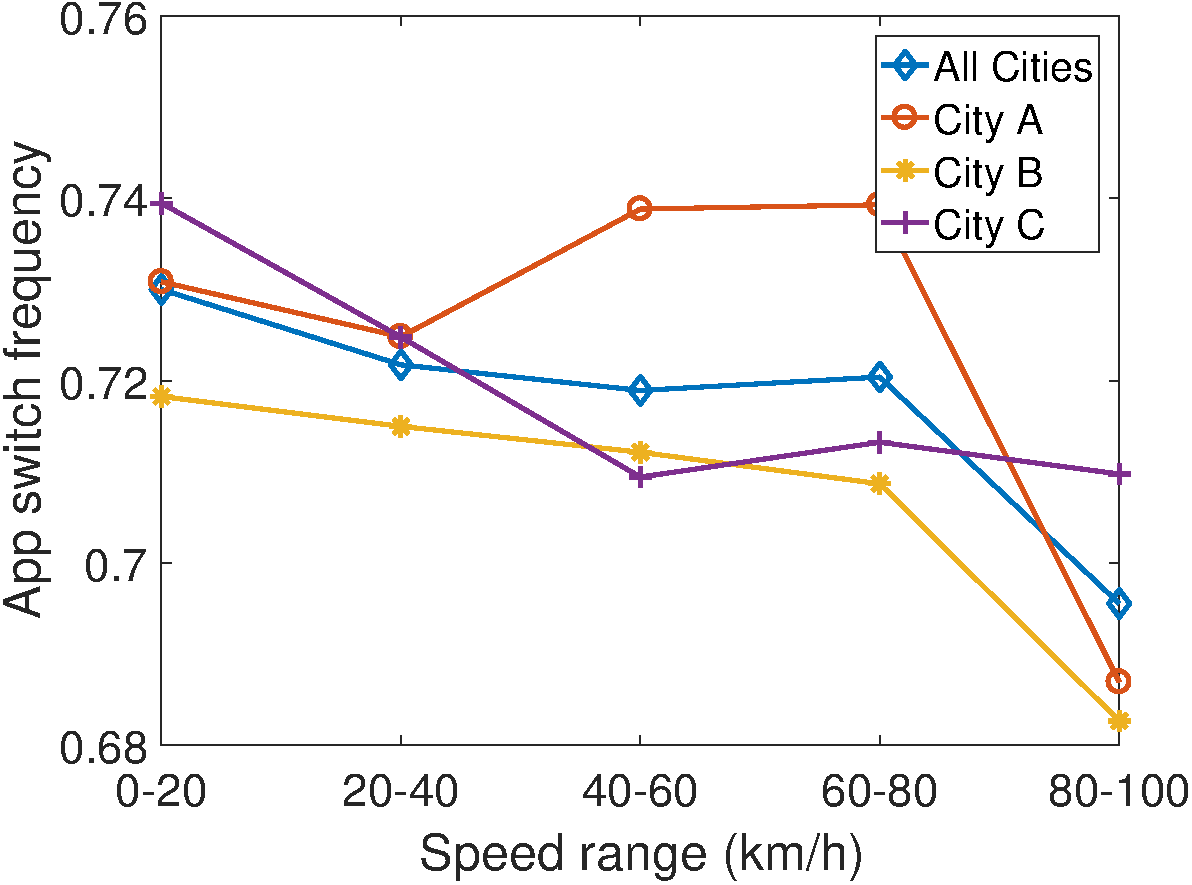
\includegraphics[width=0.48\linewidth]{./figures/app_switch_frequency_line_8_6.pdf}}
		\subfigure[App category switch frequency\label{fig:switch_app_category}]{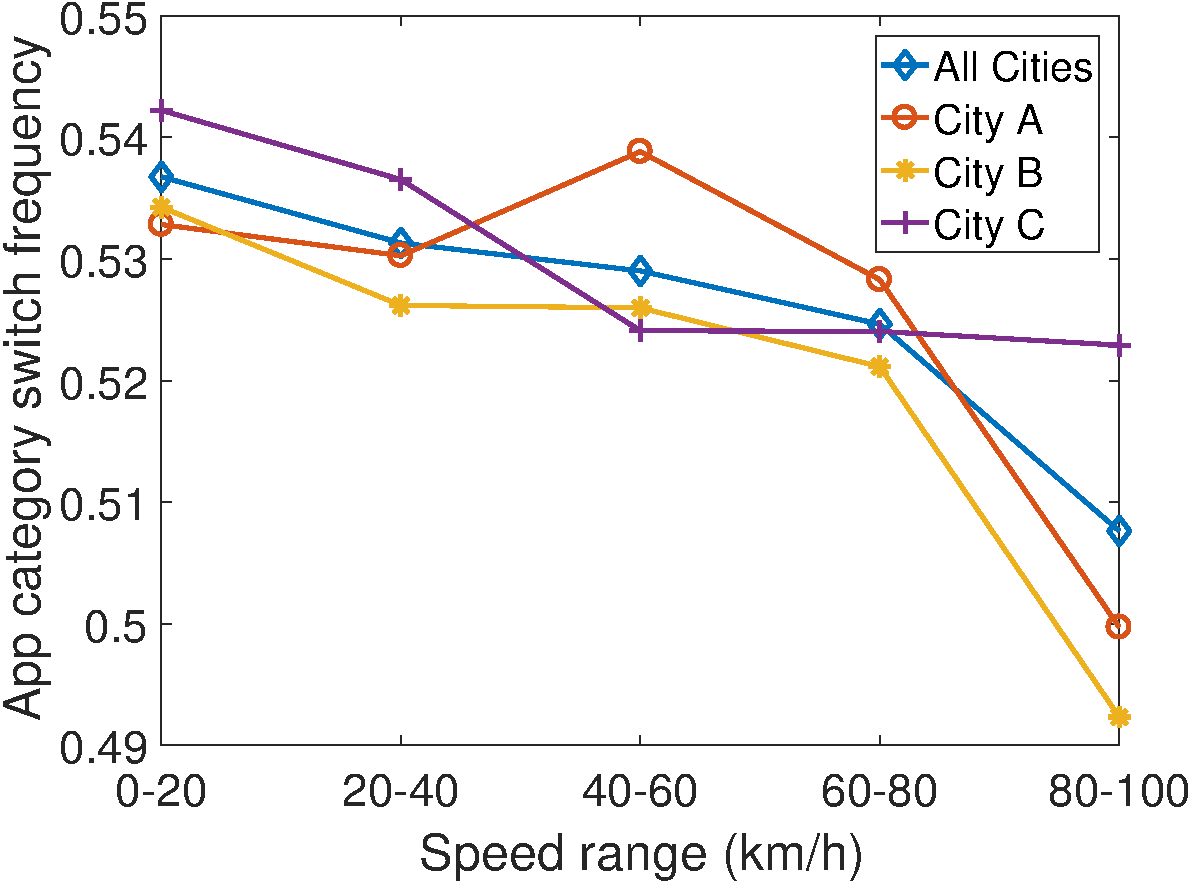
\includegraphics[width=0.48\linewidth]{./figures/app_category_switch_frequency_line_8_6.pdf}}
    \caption{Correlation of user speed and the frequencies of app and app category switch}
    \label{fig:speed_app_switch}
\end{figure*}

In \autoref{fig:speed_app_switch}, we show the frequency of app switch and app category switch. They both follow the same trend that lower speed users tend to switch apps and app categories more frequently. Combined with \autoref{fig:speed_app_used}, we can reach the conclusion that although low speed users switch apps more frequently, they only switch between fewer number of apps.

\begin{figure*}
    \centering
		\subfigure[Average number of concurrently running apps\label{fig:app_overlap}]{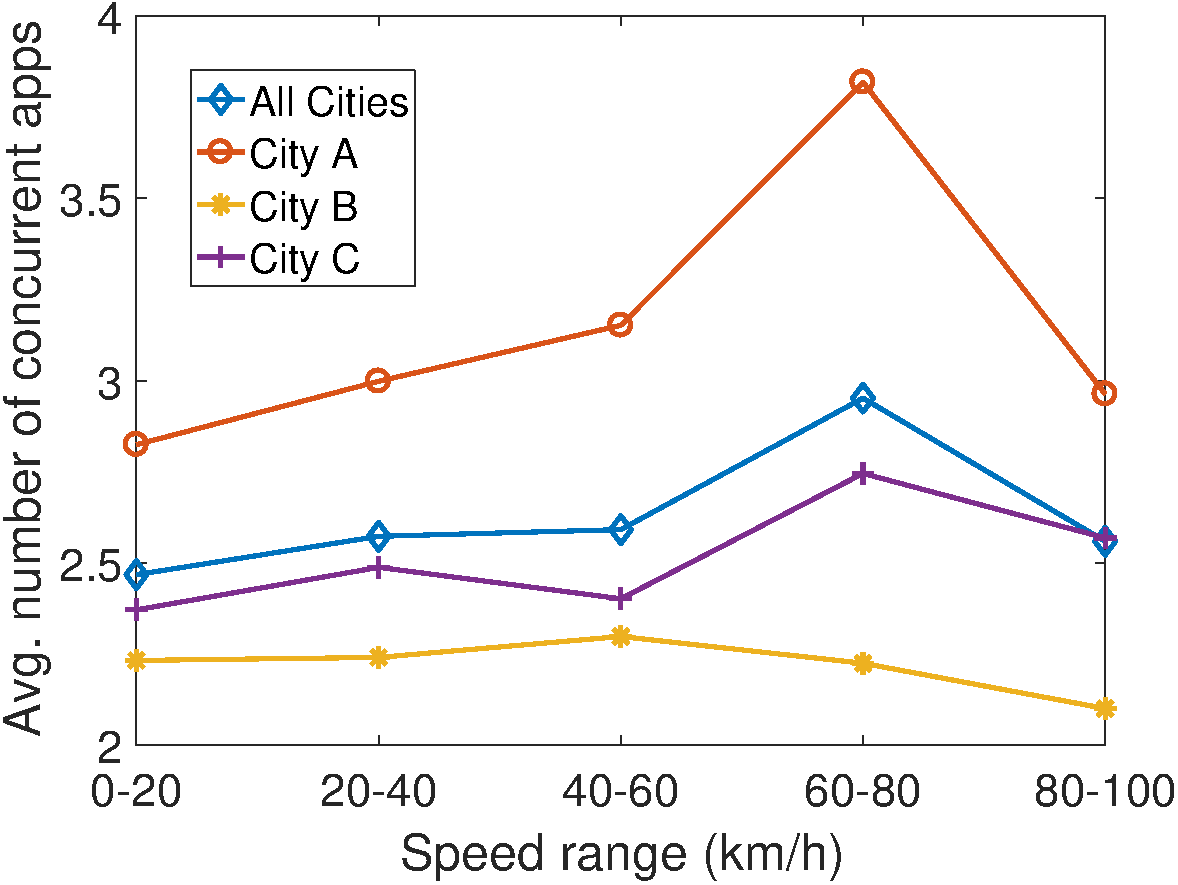
\includegraphics[width=0.48\linewidth]{./figures/app_overlap_8_6.pdf}}
		\subfigure[Average number of concurrently running app categories\label{fig:app_category_overlap}]{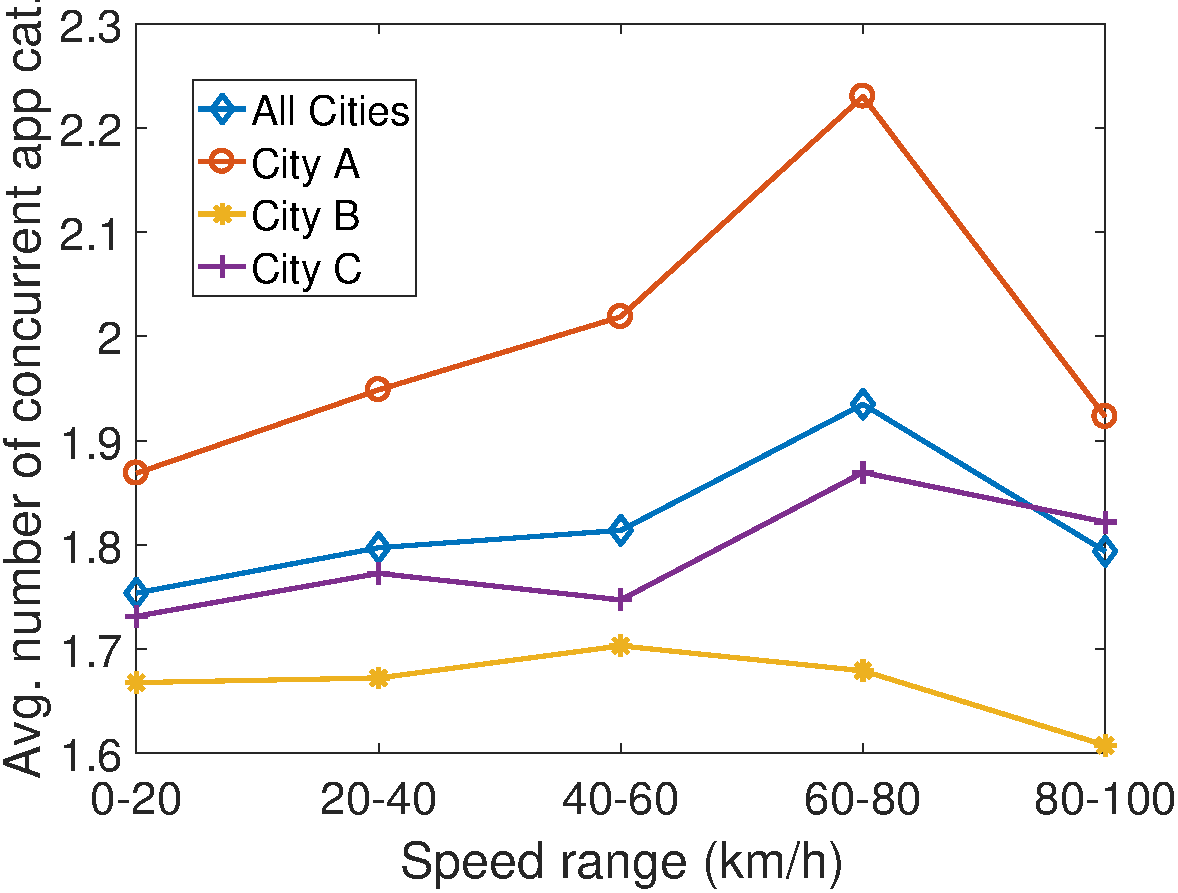
\includegraphics[width=0.48\linewidth]{./figures/app_category_overlap_8_6.pdf}}
    \caption{Correlation of user speed and the number of concurrently running apps and app categories}
    \label{fig:speed_concurrent_apps}
\end{figure*}

We then further extended our study by investigating the correlation of the number of concurrently running apps and app categories with estimated user speed. The result is shown in \autoref{fig:speed_concurrent_apps}. Although the actual launch time and close time for each running app are unavailable, we use the network access data to infer such information. For each app, we treat the time of the first data access as the launch time of an app. If the app stops accessing network for a certain period (close threshold), we record the last network access time as the close time for the app. We chose 10 seconds as the close threshold to plot \autoref{fig:speed_concurrent_apps}, but we had tested various close threshold and found similar trends except differences in value. In most cities, the peak happens at the 60-80 km/h and decreases as the speed keeps increasing. Currently, we do not have a direct explanation for this trend. We will continue this study in future works.

%\subsubsection{App Category Information}

%In this section,
In the last, we further investigated the trend of the contribution of various app categories on the total mobile data access as the user speed increases.
The contribution was defined as the mobile data access of one category versus all categories.
%However, the volume of data for each category is not even, among all 19 categories, we only interested in the
Focusing on apps that contributed the most to the total mobile data access volume,
we selected the top 8 app categories.
The correlation between the user speed and the contribution of each category is shown in \autoref{fig:speed_appcat}.
%Note that we do not show the correlation for each individual city because for some app categories there is not sufficient data to show a clear trend.

%\subsubsection{Impact of speed on each smartphone app category}

\begin{figure*}
    \centering
    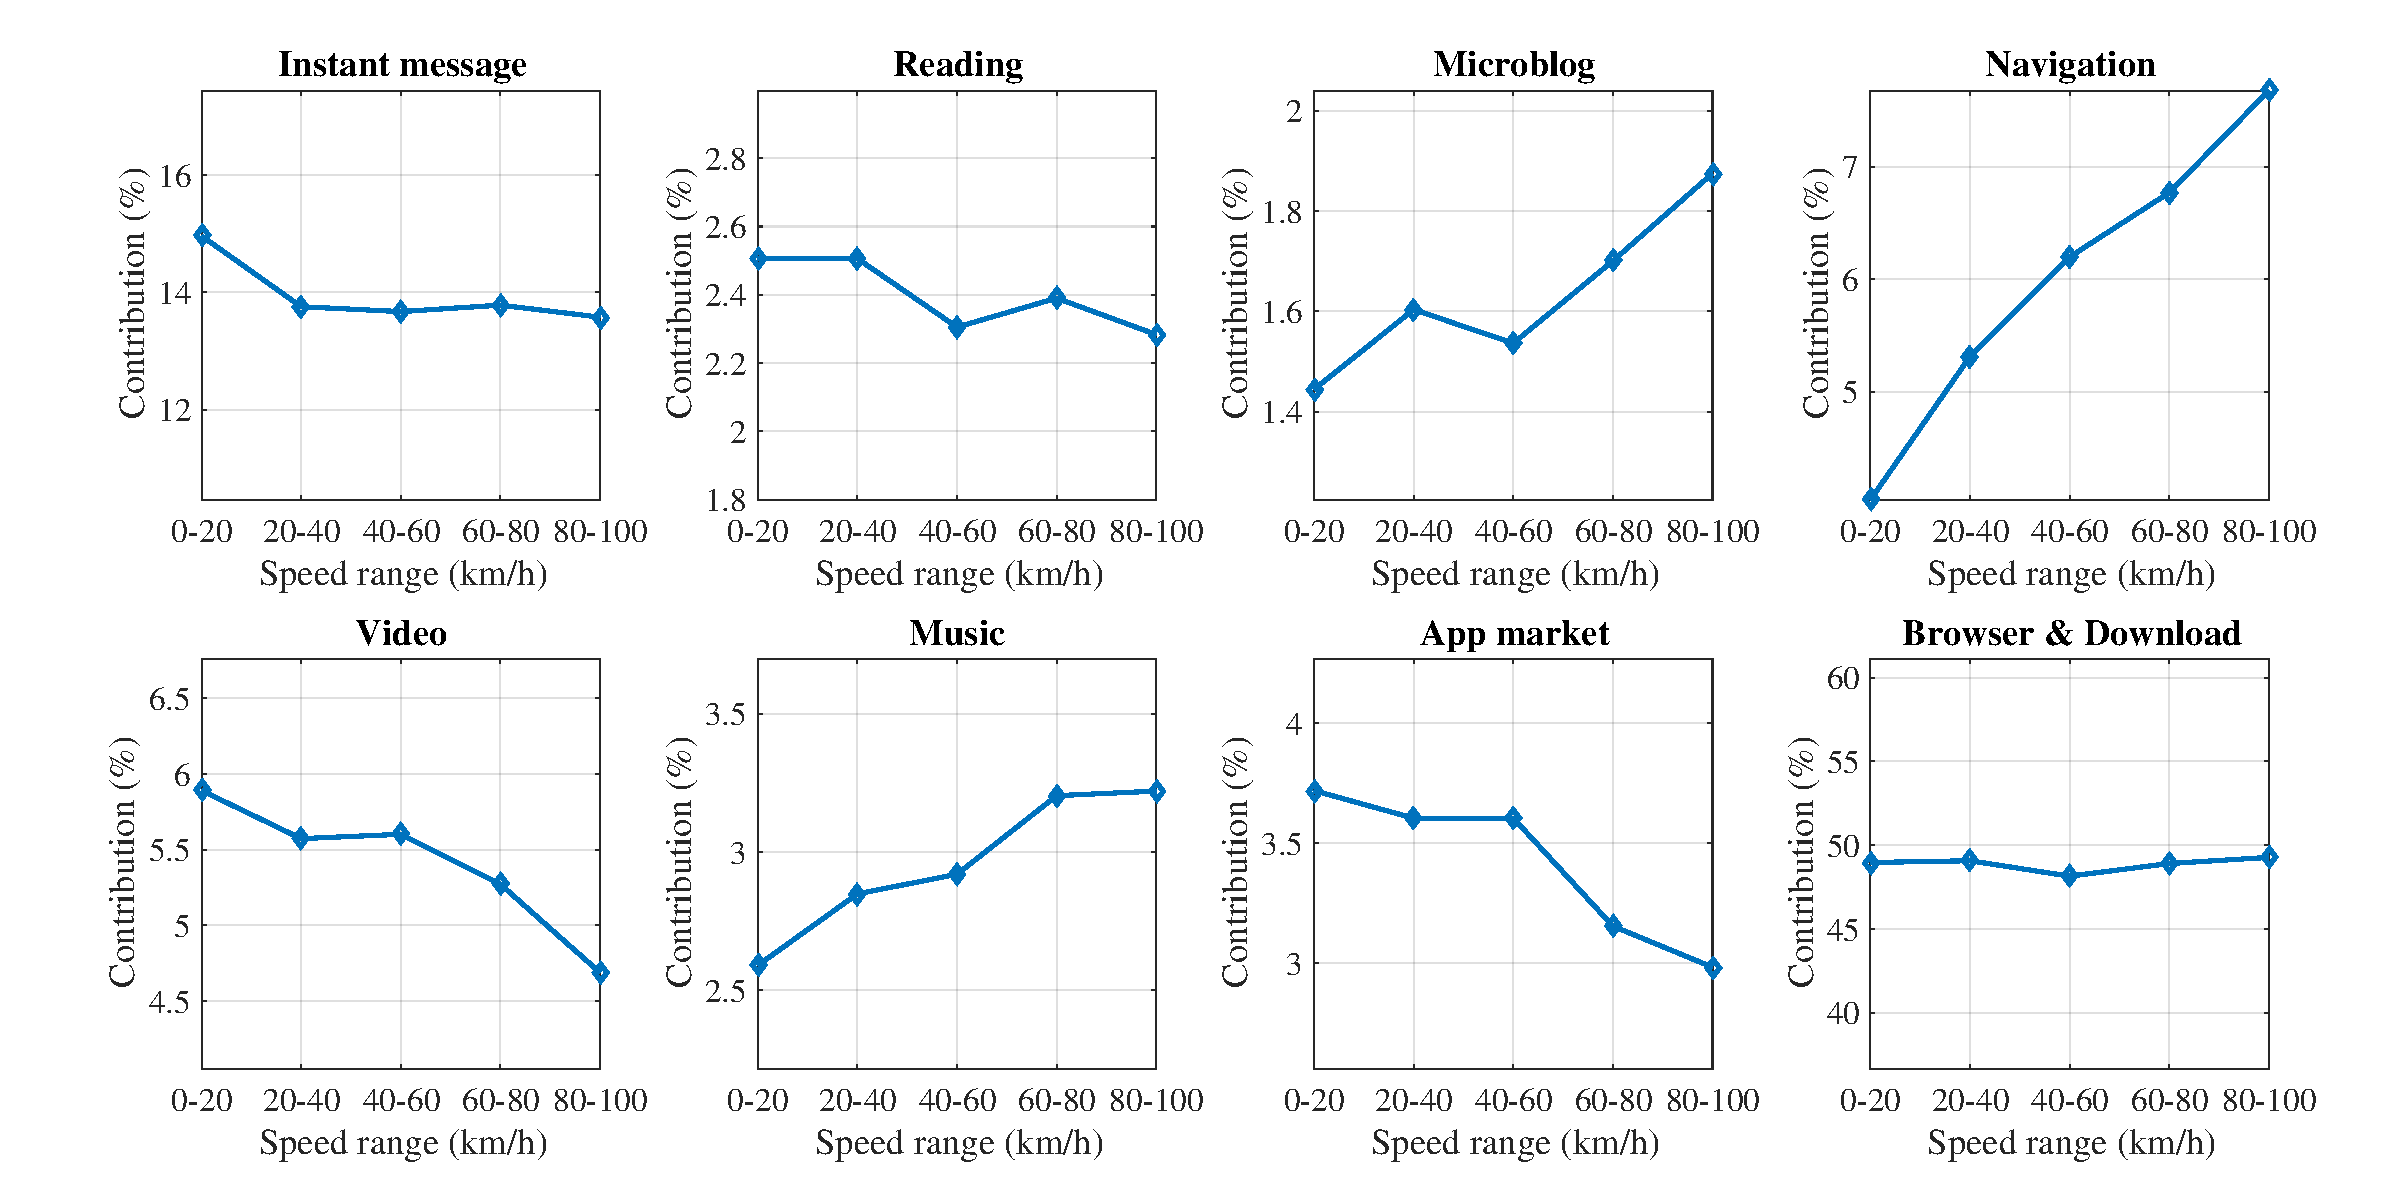
\includegraphics[width=\linewidth,height=3in]{./figures/large_font/speed_appcat.pdf}
    \vspace{-0.3in}
    \caption{Correlation of user speed and contribution of app categories.}
    \label{fig:speed_appcat}
\end{figure*}

Among the top 8 categories, Microblog, Navigation and Music show a clear upward trend as the speed increases.
The impact of navigation has the most steady increase due to the increased needs for such apps when driving.
The impact almost doubles for users with speed estimates of 80-100 km/h compared to users with speed estimates of 0-20 km/h.
Instant message, Video and App market show a downward trend as the speed increases.
The reason could be the users are cost sensitive and strictly control the data usage for large app downloading and video streaming.
Browser \& Downloading and Reading show a quite stable impact that does not change a lot as the speed increases.








\section{Conclusions}\label{conclusion}

In this paper, we studied the correlation between user mobility and app usage patterns.
In particular, we focused on users' moving speed as the key mobility metric. 
%We identified correlation between user speed and the app usage patterns for different categories of apps. 
A key challenge addressed by our methodology is to estimate speeds accurately with high confidence and reliability. 
We verify our methodology with out of sample data. The results shows great improvement in estimation accuracy.
Based on the speed estimations, we are able to reveal the correlation of user mobility with mobile data usage patterns 
including the data volume, the data access frequency, and the traffic share of apps on the total mobile data traffic. 
Results showed that with users that have high speed estimation tend to user smartphone more frequently and 
generate more traffic on the mobile data network. 
Furthermore, the user speed also played an important role in the contribution of each smartphone app categories on the total mobile data traffic. 

\bibliographystyle{ACM-Reference-Format}
\bibliography{refs}

\end{document}
